\section{Úvod do problematiky}

V oblasti finančných technológií dochádza v posledných rokoch k výraznému pokroku,
ktorý je poháňaný rastúcou automatizáciou a digitalizáciou procesov. Fakturácia a
správa finančných dokumentov patria medzi kľúčové oblasti, kde je možné využiť
moderné technológie na zefektívnenie a zjednodušenie práce. V tradičných fakturačných
systémoch sa používatelia často stretávajú s komplikovanými rozhraniami a manuálnym
vyhľadávaním informácií, čo môže viesť k časovým stratám a zvýšenému riziku chýb.

Jedným z možných riešení, ktoré by mohlo priniesť významné zlepšenie, je
integrácia inteligentných asistentov využívajúcich umelú inteligenciu a
technológie spracovania prirodzeného jazyka (Natural Language Processing, NLP).
S príchodom pokročilých modelov spracovania prirodzeného jazyka, ako sú Large Language
Models (\gls{llm}), sa otvorili nové možnosti interakcie medzi používateľom a systémom.
Tieto modely dokážu spracovávať dotazy používateľov v prirodzenom jazyku, interpretovať
ich význam a poskytovať relevantné odpovede bez potreby špecifického technického slovníka
alebo komplikovaného zadávania príkazov.

Jednou z výziev pri implementácii takýchto riešení je správna integrácia \gls{llm}
modelov s existujúcimi fakturačnými systémami, kde je potrebné zabezpečiť plynulý
tok dát, efektívne spracovanie dotazov a vysokú presnosť odpovedí. Kľúčovou otázkou
je tiež výber vhodného modelu, ktorý dokáže pracovať s finančnými údajmi a
správne interpretovať špecifické požiadavky používateľov.

Táto diplomová práca sa zaoberá návrhom a implementáciou inteligentného
finančného asistenta FinanceGPT, ktorý bude využívať \gls{llm} modely na
spracovanie dotazov používateľov v prirodzenom jazyku a poskytovať relevantné
odpovede týkajúce sa fakturácie a finančných dokumentov. FinanceGPT bude integrovaný
s fakturačnou aplikáciou vytvorenou v rámci bakalárskej práce, čo umožní
využitie existujúcej infraštruktúry a poskytne základ pre rozšírenie o nové
funkcionality. Hlavným cieľom je vytvoriť systém, ktorý používateľom poskytne
intuitívny a efektívny spôsob interakcie s ich finančnými údajmi.

\subsection{Trendy vo finančných technológiách}

Oblasť finančných technológií (FinTech) zaznamenala v posledných rokoch výrazný rast,
čo dokladujú viaceré správy renomovaných spoločností. KPMG vo svojej analýze The Pulse
of Fintech H1 2021 zdôrazňuje význam inovácií v platobných systémoch, blockchain
riešeniach a využití umelej inteligencie na automatizáciu opakovaných úkonov. Digitalizácia
v oblasti financií sa prejavuje najmä prechodom od tradičných papierových procesov
k elektronickým riešeniam, ktoré sú rýchlejšie a znižujú chybovosť.

V kontexte malých a stredných podnikov (SME - Small and Medium Enterprises) sa
FinTech technológie sústreďujú na zjednodušenie riadenia finančných tokov, správu
faktúr či platobné služby. Stále dôležitejšou témou sa stáva bezpečnosť a
ochrana údajov, keďže práve v oblasti financií sa narába s citlivými informáciami.
Tieto faktory následne ovplyvňujú smerovanie výskumu a vývoja v danom sektore.

Práve v tomto kontexte nadobúda mimoriadny význam automatizácia spracovania
finančných dokumentov s využitím umelej inteligencie. Konverzační asistenti schopní
porozumieť prirodzenému jazyku predstavujú prirodzenú evolúciu FinTech nástrojov,
ktoré umožňujú malým a stredným podnikateľom efektívne pracovať s finančnými
dátami bez nutnosti technickej expertízy~\cite{atkinson2025}.

% https://kpmg.com/sk/sk/home/media/press-releases/2021/08/financne-technologie-zaznamenali-rekordny-zaujem-investorov.html

\subsection{Doména finančných dokumentov a výzvy pri ich správe}

Jedným z tradičných problémov finančných oddelení a účtovných spoločností je
manuálna správa faktúr a ďalších finančných dokumentov. Často ide o časovo náročné
aktivity zahŕňajúce vyhľadávanie faktúr v archívoch, manuálne kopírovanie údajov
a zisťovanie stavu úhrad. Európska komisia vo svojej správe k elektronickej fakturácii
(eInvoicing) uvádza, že zefektívnenie týchto procesov môže viesť k výrazným
úsporám nákladov, skráteniu času spracovania faktúr a zníženiu miery chýb.
% https://ec.europa.eu/digital-building-blocks/sites/display/DIGITAL/What+is+eInvoicing

% https://ec.europa.eu/digital-building-blocks/sites/display/DIGITAL/What+are+the+benefits+of+eInvoicing
Ďalšou výzvou je vhodná organizácia a archivácia elektronických dokumentov. Pri
rýchlej expanzii digitálnych nástrojov môže vznikať problém s integritou dát
alebo s ich redundanciou. Prehľadné a centralizované riešenia dokážu zjednodušiť vyhľadávanie
požadovaných informácií a minimalizovať manuálne úkony.

Špecifickou výzvou pre fakturačné systémy je pritom samotná interakcia používateľa
s dátami — tradičné riešenia ponúkajú len statické filtre a prehľadávacie formuláre,
ktoré od používateľa vyžadujú znalosť štruktúry systému. Inteligentný asistent pracujúci
s prirodzeným jazykom tento problém odstraňuje tým, že prekladá voľne
formulované otázky priamo do databázových operácií, čím znižuje kognitívnu záťaž používateľa~\cite{zhao2023survey}.

\subsection{Vývoj v oblasti spracovania prirodzeného jazyka (NLP)}

Spracovanie prirodzeného jazyka (NLP) prešlo dlhým vývojom, od štatistických metód
a jednoduchých pravidlových systémov k sofistikovaným modelom využívajúcim hlboké
neurónové siete. Medzi prelomové práce patrí napríklad BERT (Bidirectional Encoder
Representations from Transformers) vyvinutý výskumníkmi v spoločnosti Google. Moderné
NLP modely vďaka kontextuálnemu spracovaniu slov poskytujú lepšie výsledky pri porozumení
textu a zvládajú zložitejšiu interpretáciu dopytov.

V posledných rokoch sa pozornosť sústreďuje na tzv. Large Language Models (\gls{llm}),
ktoré disponujú vysokou kapacitou parametrov a umožňujú, aby model dokázal generalizovať
vedomosti z obrovských textových korpusov. Tieto modely sú schopné generovať
zrozumiteľné texty a spracúvať dotazy v prirodzenom jazyku na vysokej úrovni.

V oblasti finančných aplikácií sa \gls{llm} modely osvedčujú najmä pri spracovaní
neštruktúrovaných dotazov nad štruktúrovanými dátami — napríklad pri prevode otázky
v prirodzenom jazyku na databázový dopyt (Text-to-SQL). Rothman (2023)
zdôrazňuje, že architektonický základ Transformer modelov im umožňuje porozumieť doménovej
terminológii a kontextovým väzbám, čo je predpokladom ich úspešného nasadenia v
špecializovaných systémoch, akým je FinanceGPT~\cite{rothman2023transformers}.

\subsection{Potenciál \gls{llm} modelov vo finančnom sektore}

V oblasti finančných služieb sa \gls{llm} modely úspešne využívajú pri automatickej
tvorbe reportov, sumarizácii dôležitých faktov a v chatbot riešeniach pre
klientsku podporu. Mnohé účtovné softvéry ako QuickBooks, Xero či FreshBooks sa
snažia postupne integrovať konverzačné prvky a inteligentné asistentovstvo do
svojich platforiem.

% https://cdn.openai.com/papers/gpt-4.pdf
% (AI Assistent iba v USA) https://quickbooks.intuit.com/ai-accounting/
% https://www.xero.com/just-ask-xero/
% https://www.xero.com/media-releases/xero-unveils-its-ai-vision-to-reimagine-small-business-accounting/
% https://www.qualified.com/plus/articles/freshbooks-leans-on-piper-the-ai-sdr-to-boost-conversions-and-enhance-the-buyer-experience

Modely typu GPT-4 či GPT-o1 od spoločnosti OpenAI demonštrujú schopnosti poradiť si
s kontextom veľkého rozsahu a generovať odpovede, ktoré môžu znížiť
administratívnu záťaž finančných pracovníkov. Asistent FinanceGPT v tomto kontexte
môže využívať silu \gls{llm} nielen na interpretáciu ľudských dotazov v
prirodzenom jazyku, ale aj na navrhovanie ďalších krokov pri správe faktúr či príprave
reportov.

Veľké jazykové modely (\gls{llm}) predstavujú prelom v oblasti umelej
inteligencie, pričom ich architektúra umožňuje spracovávať a generovať text na úrovni
blízkej ľudskému porozumeniu~\cite{zhao2023survey}. Vo finančnom sektore sa ich
potenciál naplno prejavuje pri automatizácii analytických úloh, ako je klasifikácia
výdavkov, interpretácia cash-flow či generovanie finančných reportov. Podľa Atkinson-Abutridy
(2023) je jednou z hlavných výhod \gls{llm} ich schopnosť kontextuálneho
porozumenia špecifickej doménovej terminológii, čo výrazne znižuje chybovosť pri interpretácii
požiadaviek používateľov~\cite{atkinson2023llm}. Nasadenie týchto modelov v
systémoch, akým je FinanceGPT, používateľom umožňuje klásť zložité otázky o
svojich financiách v prirodzenom jazyku bez nutnosti ovládania databázových
jazykov alebo zložitého filtrovania v systéme.

\subsection{Ciele a prínosy projektu FinanceGPT}

Hlavným cieľom projektu FinanceGPT je priniesť inteligentného asistenta, ktorý
zjednoduší interakciu s finančnými údajmi pre používateľov, či už ide o manažérov,
účtovníkov alebo podnikateľov v SME segmente. Očakávaným prínosom je rýchlejšie a
intuitívnejšie vyhľadávanie informácií o príjmoch a výdavkoch, generovanie
súhrnných správ a vizualizácií umožňujúcich lepší prehľad o financiách.

V porovnaní s existujúcimi riešeniami na trhu chce FinanceGPT využiť aktuálne
poznatky v oblasti spracovania prirodzeného jazyka, ktoré umožnia učiť sa z rôznych
typov dokumentov a kontextov. Vyžaduje si to však riešenie viacerých výziev, predovšetkým
integráciu s existujúcimi systémami, zabezpečenie ochrany citlivých údajov a
vhodné nastavenie NLP modelu tak, aby bol schopný zvládať špecifickú terminológiu
finančného sektora.

Technologickým základom projektu FinanceGPT je webová aplikácia vyvinutá v rámci predchádzajúcej
bakalárskej práce autora~\cite{ruby2025}. Táto aplikácia, implementovaná v rámci Ruby
on Rails, pokrývala komplexnú správu faktúr vrátane automatického doplňovania
údajov o subjektoch z verejného Registra právnických osôb (RPO) a správu
bankových spojení. Existujúci dátový model obsahuje tabuľky \texttt{invoices}, \texttt{entities}
a \texttt{bank\_details}, ktoré tvoria doménový základ, nad ktorým asistent FinanceGPT
operuje.

Táto diplomová práca teda nepristupuje k problému od nuly, ale rozširuje funkčný
a v praxi overený systém o vrstvu inteligencie. Takýto prístup umožnil sústrediť vývojové
úsilie na samotnú LLM integráciu namiesto budovania infraštruktúry od základov,
čo je v kontexte agilného vývoja softvéru považované za zásadnú výhodu~\cite{ruby2025}.

\section{Analýza súčasného stavu}

Táto kapitola analyzuje oblasť správy finančných dokumentov z dvoch perspektív.
Prvá línia skúma existujúce fakturačné systémy na slovenskom a zahraničnom trhu
a hodnotí ich z hľadiska automatizácie, integrovateľnosti a podpory konverzačných
rozhraní. Druhá línia mapuje technologické predpoklady pre integráciu veľkých
jazykových modelov do webového prostredia — od evolúcie NLP metód cez
architektúru Transformer až po regulačné požiadavky finančnej domény. Výsledky analýzy
slúžia ako podklad pre návrh systému v nasledujúcej kapitole.

% ============================================================
\subsection{Prehľad existujúcich riešení pre správu faktúr}

Pre hodnotenie existujúcich systémov boli zvolené kritériá relevantné pre
konverzačné spracovanie finančných dát: miera automatizácie, dostupnosť
otvoreného API, úroveň integrácie umelej inteligencie (vrátane \gls{llm}), podpora
konverzačného rozhrania a dostupnosť pre slovenský trh.

% ============================================================
\subsubsection{Slovenské a zahraničné fakturačné systémy}

Na slovenskom trhu patria medzi rozšírené riešenia platformy Superfaktúra, Fakturovo,
Kros a FakturaOnline. Tieto systémy poskytujú štandardnú fakturačnú agendu vrátane
sledovania stavu úhrad a štatistických reportov, pričom žiadny z nich v
súčasnosti neimplementuje konverzačné rozhranie na báze veľkého jazykového
modelu.

Na zahraničnom trhu boli analyzované systémy Xero, QuickBooks, FreshBooks, Vic.ai,
Abe.ai a Bookkeeping.ai. Tieto platformy predstavujú rozmanité prístupy k integrácii
umelej inteligencie — od detekcie anomálií a kategorizácie výdavkov až po experimentálne
konverzačné rozhrania. Prehľad kľúčových charakteristík je zhrnutý v~tabuľke~\ref{tab:fakturacne-systemy}.

\begin{table}[htbp]
	\centering
	\caption{Porovnanie vybraných fakturačných systémov z hľadiska AI a
	konverzačného rozhrania}
	\label{tab:fakturacne-systemy} \resizebox{\textwidth}{!}{%
	\begin{tabular}{|l|l|c|c|c|c|}
		\hline
		\textbf{Systém}            & \textbf{Typ AI}          & \textbf{LLM} & \textbf{Konv. rozhranie} & \textbf{Otvorené API} & \textbf{SK trh} \\
		\hline
		Superfaktúra / Fakturovo   & Štatistické reporty      & Nie          & Nie                      & Áno                   & Áno             \\
		Xero (Just Ask Xero)       & ML + NLP                 & Čiastočne    & Obmedzene                & Áno                   & Nie             \\
		QuickBooks (Intuit Assist) & GenAI (GenOS)            & Áno          & Áno                      & Áno                   & Nie             \\
		FreshBooks (Addy / Piper)  & AI agent (predajný)      & Nepriamo     & Nie                      & Áno                   & Nie             \\
		Vic.ai                     & Špecializovaná AI        & Nie          & Nie                      & Áno                   & Nie             \\
		Abe.ai / Yodlee            & Konverzačné bankovníctvo & Čiastočne    & Áno                      & Áno                   & Nie             \\
		Bookkeeping.ai (Paula)     & LLM (GPT-4)              & Áno          & Áno                      & Obmedzene             & Nie             \\
		\hline
	\end{tabular}%
	}
\end{table}

Z analýzy vyplývajú tri kľúčové pozorovania. Po prvé, slovenské fakturačné systémy
zatiaľ neponúkajú AI-driven konverzačné rozhranie, čím vzniká priestor pre
riešenie tejto medzery na lokálnom trhu. Po druhé, systémy ako QuickBooks a
Bookkeeping.ai potvrdzujú technickú realizovateľnosť integrácie \gls{llm} do finančnej
domény — ich architektúry (GenAI vrstva nad existujúcimi dátami, Tool Calling,
Text-to-SQL) naznačujú smer, akým sa segment vyvíja. Po tretie, kľúčovým limitom
väčšiny pokročilých zahraničných platforiem zostáva absencia natívnej podpory
slovenského jazyka a závislosť od uzavretého ekosystému poskytovateľa.

% ============================================================
\subsubsection{AI agenti vs.\ AI asistenti vo finančnej doméne}

V odbornej literatúre a priemyselných štandardoch sa striktne rozlišuje medzi dvoma
paradigmami inteligentných systémov, pričom ich rozdiel spočíva predovšetkým v
miere proaktivity a autonómie~\cite{ibm2024}.

\begin{itemize}
	\item \textbf{AI asistent (reaktívny systém):} Vykonáva úlohy výhradne na
		požiadanie používateľa. Reaguje na zadané vstupy v prirodzenom jazyku, no
		sám nevyvíja iniciatívu. Typickým príkladom je konverzačné rozhranie, ktoré
		odpovedá na otázky alebo agreguje dáta na základe explicitného pokynu.

	\item \textbf{AI agent (autonómny systém):} Proaktívny systém so stanoveným
		komplexným cieľom, ktorý sa ho snaží dosiahnuť autonómne s využitím dostupných
		prostriedkov a nástrojov. Je schopný viac-krokového plánovania, vlastného rozhodovania
		a vykonávania akcií bez neustáleho dohľadu~\cite{zhao2023}.
\end{itemize}

Toto rozlíšenie má priamy regulačný a bezpečnostný dosah vo finančnej doméne.
Autonómne agentné systémy, ktoré by mohli napríklad proaktívne odosielať faktúry alebo
modifikovať finančné záznamy bez explicitného príkazu používateľa, podliehajú
prísnejším požiadavkám na transparentnosť a audit podľa EU AI Act. Systémy reaktívneho
charakteru, kde je každá akcia explicitne iniciovaná používateľom, naopak spadajú
do kategórie obmedzeného rizika.

% ============================================================
\subsection{Technologické možnosti}

Táto diplomová práca koncepčne nadväzuje na výsledky predchádzajúcej bakalárskej
práce~\cite{gasparovic2023}, v rámci ktorej bol vybudovaný základný technologický
zásobník: backend na frameworku \textbf{Ruby on Rails} a relačná databáza \textbf{PostgreSQL}.
Táto voľba sa v predchádzajúcej fáze projektu ukázala ako efektívna vďaka návrhovému
vzoru MVC a silnému objektovo-relačnému mapovaniu (ORM) prostredníctvom knižnice ActiveRecord,
čo je kritické aj pre aktuálnu fázu pri bezpečnom spracovávaní finančných entít~\cite{ruby2025}.

Výzva tejto diplomovej práce spočíva v rozšírení tradičného webového prístupu o
inteligentnú konverzačnú vrstvu. Integrácia veľkých jazykových modelov (\gls{llm})
do existujúcej Rails architektúry vyžaduje analýzu viacerých technologických
aspektov. Na rozdiel od štandardného vývoja, kde programátor explicitne definuje
všetky stavy a prechody aplikácie, využitie \gls{llm} vnáša do systému prvok
nedeterminizmu. Z tohto dôvodu je potrebné vyhodnotiť samotné jazykové modely,
spôsoby ich bezpečného prepojenia s relačnou databázou, metódy spracovania prirodzeného
jazyka a vhodné vizualizačné nástroje.

% ============================================================
\subsection{Technologické východiská a spracovanie prirodzeného jazyka}

\subsubsection{Evolúcia metód NLP a architektúra Transformer}

Spracovanie prirodzeného jazyka (NLP) prešlo za posledné dve desaťročia zásadnou evolúciou.
Klasické pravidlové a štatistické metódy — tokenizácia, lemmatizácia,
rozpoznávanie pomenovaných entít (NER) a syntaktická analýza — umožňili
počítačom analyzovať štruktúru textu. Ich schopnosť porozumieť kontextu dlhých sekvencií
a zachytiť sémantické závislosti medzi vzdialenými slovami bola však principiálne
obmedzená.

Prelomom bolo zavedenie rekurentných neurónových sietí (RNN), ktoré zaviedli
koncept sekvenčnej pamäte. RNN dokázali zachytávať závislosti medzi tokenmi v textovej
sekvencii, avšak trpeli tzv. problémom miznúceho gradientu — pri dlhých sekvenciách
model strácal kontext z počiatočných tokenov. Architektúry LSTM tento nedostatok
čiastočne adresovali, no fundamentálna neefektívnosť sekvenčného spracovania pretrvávala~\cite{lipton2015critical}.

Zásadným prelomom bol príchod architektúry Transformer (Vaswani et al., 2017),
ktorá nahradila sekvenčné spracovanie mechanizmom \textit{self-attention}. Ten
umožňuje modelu paralelne vyhodnocovať vzťahy medzi ľubovoľnými dvoma tokenmi
vstupu bez ohľadu na ich vzájomnú vzdialenosť v sekvencii. Táto vlastnosť sa stala
základom pre škálovanie modelov do veľkostí, pri ktorých sa objavujú tzv. emergentné
schopnosti — vrátane zero-shot a few-shot učenia. Práve tieto vlastnosti sú
kľúčové pre konverzačné systémy vo finančnej doméne, kde model musí z voľného textu
spoľahlivo rozlíšiť zámer používateľa a dynamicky volať vhodné systémové nástroje~\cite{vaswani2017attention,
zhao2023survey}.

% ============================================================
\subsubsection{Veľké jazykové modely (LLM) a ich parametre}

Pri integrácii \gls{llm} do fakturačného systému je výber vhodného modelu podmienený
súborom kritérií, ktoré vychádzajú z požiadaviek domény:

\begin{enumerate}
	\item \textbf{Podpora volania externých nástrojov (Tool Calling):} Schopnosť
		modelu generovať štruktúrovaný výstup (JSON) pre volanie preddefinovaných
		funkcií backendu je kľúčová pre deterministické prepojenie s databázovými
		operáciami.

	\item \textbf{Podpora slovenského jazyka:} Pre aplikáciu určenú slovenským
		používateľom je nevyhnutná dostatočná jazyková kompetencia vrátane odbornej
		finančnej terminológie.

	\item \textbf{Bezpečnosť a ochrana súkromia:} Pri spracovaní citlivých
		finančných dát je zásadné, aby zmluvné podmienky poskytovateľa vylučovali využitie
		zákazníckych dát na ďalšie trénovanie modelov, v súlade s požiadavkami GDPR.

	\item \textbf{Náročnosť integrácie:} Dostupnosť SDK, API a knižníc kompatibilných
		s frameworkom Ruby on Rails priamo ovplyvňuje implementačnú náročnosť.

	\item \textbf{Latencia a prevádzkové náklady:} Rýchlosť odpovedí a cena za
		spracované tokeny sú prevádzkovými faktormi, ktoré ovplyvňujú použi\-teľnosť v
		produkčnom prostredí.
\end{enumerate}

\vspace{1em}

\textbf{Mechanizmus Tool Callingu}

Tool Calling (funkčné volanie) je rozhranie, ktoré umožňuje vývojárovi poskytnúť jazykovému
modelu zoznam dostupných funkcií backendu spolu s ich očakávanými argumentmi vo formáte
JSON Schema. Model analyzuje používateľov dopyt a namiesto voľného textu
vygeneruje presne štruktúrovaný JSON objekt s parametrami pre volanie konkrétnej
funkcie~\cite{ruby2025}. Tento mechanizmus prináša tri architektonické výhody: (1)
oddelenie logiky od generovania — model nespúšťa operácie priamo, iba ich inštruuje;
(2) bezpečnostnú izoláciu — do databázy sa dostávajú len validované parametre, nie
surový SQL; (3) možnosť prepojenia textovej odpovede s vizualizačnými príkazmi
pre frontend.

\vspace{1em}

Na trhu sú v súčasnosti dostupné tri hlavné kategórie modelov relevantných pre túto
doménu:

\begin{itemize}
	\item \textbf{Komerčné frontier modely} (napr. OpenAI GPT, Anthropic Claude): vynikajú
		presnosťou pri generovaní štruktúrovaného výstupu, natívnou podporou Tool
		Callingu a kompetenciou v slovenskom jazyku. Nevýhodou je nutnosť odosielania
		databázovej schémy na externé servery poskytovateľa, čo si vyžaduje
		doplnkovú bezpečnostnú vrstvu.

	\item \textbf{Open-source modely} (napr. Meta LLaMA): umožňujú plne lokálne
		nasadenie, čo eliminuje riziko úniku dát k tretím stranám. Pri komplexných
		zero-shot úlohách v menšinových jazykoch a striktnom JSON formátovaní však
		zaostávajú za komerčnými alternatívami. Lokálne nasadenie navyše vyžaduje vlastnú
		hardvérovú infraštruktúru s GPU akcelerátormi.

	\item \textbf{Špecializované finančné modely}: optimalizované pre konkrétnu doménu,
		avšak zvyčajne bez všeobecných konverzačných schopností a s obmedzenou
		podporou slovenčiny.
\end{itemize}

% ============================================================
\subsubsection{Regulačné a bezpečnostné požiadavky na spracovanie finančných dát}

\paragraph{Správa faktúr a ochrana osobných údajov (GDPR)}

Z hľadiska finančnej legislatívy podlieha elektronická správa a archivácia faktúr
zákonu č.~431/2002~Z.\,z.\ o účtovníctve~\cite{zakon_431_2002} a zákonu č.~222/2004~Z.\,z.\ o
dani z pridanej hodnoty~\cite{zakon_222_2004}. Tieto predpisy vyžadujú
zabezpečenie vierohodnosti pôvodu, neporušenosti obsahu a čitateľnosti faktúry počas
celej povinnej doby uchovávania.

Keďže finančné dokumenty obsahujú citlivé osobné údaje, systém musí spĺňať
požiadavky Všeobecného nariadenia o ochrane údajov (GDPR)~\cite{gdpr_2016} a
zákona č.~18/2018~Z.\,z.\ o ochrane osobných údajov~\cite{zakon_18_2018}. Pri
integrácii \gls{llm} do procesu spracovania dopytov v prirodzenom jazyku vzniká špecifické
riziko úniku identifikovateľných údajov prostredníctvom API volaní. Odporúčaným
prístupom je anonymizácia alebo pseudonymizácia osobných identifikátorov ešte
pred ich odoslaním do jazykového modelu.

\paragraph{Súlad s Aktom o umelej inteligencii (EU AI Act)}

Nariadenie Európskeho parlamentu a Rady (EÚ) 2024/1689~\cite{eu_ai_act_2024}
zavádza klasifikáciu AI systémov podľa miery rizika. Konverzačné systémy určené na
vyhľadávanie finančných informácií a sumarizáciu dát na základe údajov vložených samotným
používateľom nespadajú do kategórie vysokorizikových systémov (napr. systémy hodnotenia
úverového rizika), ale zaraďujú sa medzi systémy s obmedzeným rizikom.

Pre túto kategóriu vyplýva z Článku 50 nariadenia jedna hlavná legislatívna požiadavka:
poskytovatelia systémov umelej inteligencie určených na priamu interakciu s
fyzickými osobami musia zabezpečiť, aby boli používatelia jasne informovaní o tom,
že komunikujú s umelou inteligenciou a že generované výstupy môžu obsahovať
nepresnosti~\cite{eu_ai_act_2024}.

\paragraph{Bezpečnostné hrozby špecifické pre LLM systémy}

Integrácia veľkých jazykových modelov do produkčných systémov zavádza nové
kategórie bezpečnostných hrozieb~\cite{atkinson2025}:

\begin{itemize}
	\item \textbf{Prompt Injection:} Technika, pri ktorej útočník vloží do používateľského
		vstupu škodlivé inštrukcie s cieľom prepísať pôvodné systémové pravidlá. V
		kontexte finančného asistenta môže viesť k neautorizovanému prístupu k dátam
		iných používateľov.

	\item \textbf{Databázové zraniteľnosti (SQL Injection cez LLM):} Pri
		dynamickom generovaní SQL kódu jazykovým modelom vzniká riziko
		deštruktívnych alebo neautorizovaných príkazov. Štandardné parametrizované dopyty
		tu nie sú postačujúce a sú potrebné doplnkové kontrolné mechanizmy.

	\item \textbf{Halucinácie s dopadom na integritu dát:} Model môže vygenerovať
		syntakticky správny, ale fakticky nesprávny SQL dopyt (napr.\ referencujúci neexistujúci
		stĺpec), čo vedie k aplikačnej chybe alebo nesprávnym finančným výstupom~\cite{zhao2023survey}.
\end{itemize}

Konkrétne mechanizmy ošetrenia týchto hrozieb — vrátane guardrailingu, tenant
izolácie a exception handlingu — sú predmetom návrhu systému v nasledujúcej
kapitole.

% ============================================================
\subsection{Architektonické prístupy k integrácii LLM}

\subsubsection{Integrácia s relačnou databázou: Text-to-SQL vs.\ Tool Calling}

V súčasnom vývoji LLM agentov dominujú dva hlavné prístupy k prístupu ku
štruktúrovaným dátam.

\textbf{1. Prístup na báze volania nástrojov (Tool Calling):} Model negeneruje priamo
databázové dopyty, ale volá preddefinované funkcie aplikačného rozhrania (napr.\ get\_unpaid\_invoices()).
Výhodou je maximálna bezpečnosť — model nemá priamy prístup k databázovej schéme
a všetky operácie prechádzajú ORM vrstvou. Nevýhodou je obmedzená flexibilita:
systém dokáže odpovedať len na typy dopytov, pre ktoré bola vopred naprogramovaná
príslušná funkcia~\cite{atkinson2025}.

\textbf{2. Dynamické generovanie dopytov (Text-to-SQL):} Model vygeneruje priamy
SQL dopyt na základe poskytnutej databázovej schémy a požiadavky v prirodzenom
jazyku. Tento prístup umožňuje ad-hoc analytické otázky bez nutnosti predprogramovania
každého nového typu reportu. Hlavným kompromisom je vyššia bezpečnostná
zraniteľnosť, ktorá si vyžaduje doplnkovú ochrannú vrstvu, a závislosť kvality
výstupu od schopnosti modelu správne interpretovať databázovú schému.

Porovnanie oboch prístupov z hľadiska kľúčových kritérií je zhrnuté v tabuľke~\ref{tab:db-pristupy}.

\begin{table}[htbp]
	\centering
	\caption{Porovnanie architektonických prístupov k integrácii LLM s relačnou
	databázou}
	\label{tab:db-pristupy}
	\begin{tabular}{|l|c|c|}
		\hline
		\textbf{Kritérium}        & \textbf{Tool Calling} & \textbf{Text-to-SQL} \\
		\hline
		Flexibilita dopytov       & Nízka                 & Vysoká               \\
		Bezpečnostná zraniteľnosť & Nízka                 & Stredná–vysoká       \\
		Vývojová réžia            & Vysoká                & Nízka                \\
		Závislosť od schémy DB    & Nepriama              & Priama               \\
		Predvídateľnosť výstupu   & Vysoká                & Stredná              \\
		\hline
	\end{tabular}
\end{table}

% ============================================================
\subsubsection{Vektorové vyhľadávanie a architektúra RAG}

Bežné veľké jazykové modely nedisponujú priamym prístupom k neverejným dátam
konkrétneho používateľa. Ak sa model pokúša generovať faktické odpovede na základe
nedostatočného alebo neaktuálneho kontextu, dochádza k nežiaducemu javu
nazývanému halucinácie. V súčasnom technickom prostredí sa tento problém rieši architektúrou
RAG (Retrieval-Augmented Generation)~\cite{zhao2023survey}.

Architektúra RAG funguje v dvoch fázach. V indexovacej fáze sú časti dokumentov
(napr.\ položky faktúr, poznámky) transformované na viacdimenzionálne číselné
vektory (tzv.\ \textit{embeddings}) a uložené vo vektorovej databáze. V retrieval
fáze je pri každom dopyte vyhľadaných $k$ sémanticky najpodobnejších fragmentov,
ktoré sú pridané do kontextového okna modelu (\textit{context window}) pred samotným
generovaním odpovede. Tým sa model ukotvuje na overiteľné dáta namiesto
generovania z trénovacej pamäte~\cite{zhao2023survey}.

Dostupné riešenia pre vektorové ukladanie zahŕňajú dedikované databázy (Pinecone,
Milvus, Weaviate) a rozšírenia existujúcich relačných databáz (napr.\ rozšírenie
\texttt{pgvector} pre PostgreSQL). Dedikované vektorové databázy prinášajú optimalizovaný
výkon pri vysokom objeme vektorov za cenu pridanej architektonickej komplexnosti.
Rozšírenia existujúcich databáz naopak minimalizujú infraštruktúrnu réžiu a
umožňujú kombináciu sémantického a relačného filtrovania v rámci jednej
databázovej vrstvy, čo je výhodné pri systémoch s existujúcou relačnou schémou.

% ============================================================
\subsection{Webové technológie pre vývoj konverzačného rozhrania}

\subsubsection{Aplikačný rámec Ruby on Rails v kontexte AI integrácií}

Ruby on Rails je webový framework postavený na princípe konvencie pred konfiguráciou,
ktorý poskytuje robustné ORM mapovanie (ActiveRecord) a bohatú sadu abstrakčných
vrstiev pre vývoj databázovo orientovaných aplikácií~\cite{ruby2024agile}. Pre integráciu
konverzačného AI rozhrania sú relevantné najmä dve vlastnosti frameworku:
natívna podpora asynchrónnej komunikácie prostredníctvom technológie Hotwire (Turbo
Streams, Stimulus), ktorá umožňuje streamovanie odpovedí \gls{llm} priamo do DOM štruktúry;
a integrovaná vrstva ActiveRecord pre parametrizáciu dopytov, kľúčová pri bezpečnom
spracovaní dynamicky generovaného SQL.

Pre vývoj konverzačného rozhrania prichádzajú do úvahy dva architektonické prístupy.
\textbf{Rails monolit s Hotwire} zachováva jednotnú serverovú aplikáciu, kde
asynchrónne aktualizácie UI sú riadené Turbo Streams bez potreby oddeleného
klientskeho frameworku. Tento prístup minimalizuje počet technologických vrstiev a
uľahčuje integráciu s existujúcou aplikačnou logikou. \textbf{Rails API s
oddeleným klientskym rozhraním} (napr.\ React, Vue) ponúka vyšší stupeň voľnosti pre
interaktívne UI komponenty a jednoduchšiu integráciu moderných vizualizačných knižníc,
avšak vyžaduje zavedenie build pipeline a samostatnú správu dvoch aplikačných
vrstiev.

% ============================================================
\subsubsection{Dynamický rendering a vizualizácia údajov}

Pre vykresľovanie grafov v konverzačnom rozhraní boli posudzované štyri knižnice z
hľadiska kompatibility s ekosystémom Ruby on Rails a možnosti dynamického renderovania
asynchrónne doručených dát:

\begin{itemize}
	\item \textbf{Chart.js} — JavaScriptová knižnica pre štandardné typy grafov (stĺpcové,
		čiarové, koláčové). Vyznačuje sa priamočiarou konfiguráciou, rozsiahlou
		dokumentáciou a natívnou kompatibilitou s prostredím importmap, čo nevyžaduje
		prítomnosť Node.js build pipeline. Umožňuje dynamické generovanie
		vizualizácií na úrovni klientskej logiky.

	\item \textbf{Chartkick} — knižnica pre ekosystém Ruby on Rails poskytujúca
		view helpers na jednoriadkové generovanie grafov v ERB šablónach (napr.\ \texttt{<\%=
		bar\_chart @data \%>}). Ako vykresľovacie jadro využíva Chart.js. Je ideálna
		pre statické zobrazenie serverom predpripravených dát, no jej statická väzba na
		serverový životný cyklus komplikuje asynchrónne prekresľovanie na základe prichádzajúcich
		odpovedí z~API.

	\item \textbf{D3.js} — nízkoúrovňová knižnica poskytujúca plnú kontrolu nad
		SVG vizualizáciami. Umožňuje tvorbu komplexných a vysoko interaktívnych dátových
		reprezentácií, avšak za cenu výrazne väčšieho objemu kódu a hlbokej znalosti
		DOM manipulácie. Pre štandardizované typy finančných grafov predstavuje neúmerne
		vysokú implementačnú réžiu.

	\item \textbf{Recharts} — deklaratívna React knižnica postavená na D3.js. Predpokladá
		prítomnosť npm build pipeline a React prostredia, čo ju robí architektonicky
		nekompatibilnou s čisto serverovým Rails prístupom bez oddeleného
		klientského buildovacieho nástroja.
\end{itemize}

\vspace{1em}

% 3. Kapitola: Návrh systému
\section{Návrh systému}
Cieľom tejto kapitoly je transformovať analytické poznatky z predchádzajúcej časti
do konkrétneho architektonického a softvérového návrhu inteligentného finančného asistenta
FinanceGPT. Systém je navrhnutý ako priame funkčné rozšírenie existujúcej
webovej aplikácie pre tvorbu finančných dokumentov, pričom využíva moderné prístupy
spracovania prirodzeného jazyka a dynamického volania nástrojov (Tool Calling).

\subsection{Požiadavky na systém}
Pred samotným návrhom architektúry a databázového modelu je nevyhnutné exaktne definovať
funkčné a nefunkčné požiadavky. Tieto požiadavky vychádzajú z primárneho zadania
práce a obmedzení existujúceho kódového základu.

\subsubsection{Funkčné požiadavky}
Funkčné požiadavky definujú, aké operácie a procesy musí asistent FinanceGPT používateľovi
poskytovať. Kľúčovou vlastnosťou je schopnosť systému porozumieť voľnému textu a
autonómne zvoliť vhodný postup na získanie dát \cite{atkinson2025}. Systém spĺňa nasledujúce
funkčné požiadavky:

\begin{itemize}
	\item \textbf{Spracovanie dotazov v prirodzenom jazyku:} Systém prijíma
		textové vstupy od používateľa a prostredníctvom veľkého jazykového modelu (LLM)
		identifikuje zámer a extrahuje potrebné parametre.

	\item \textbf{Vyhľadávanie informácií o príjmoch (SQL generovanie):} Systém
		dokáže na základe dotazu vygenerovať bezpečný databázový dopyt, vykonať ho nad
		existujúcimi tabuľkami (faktúry, subjekty, bankové detaily) a vrátiť presné informácie
		o príjmoch.

	\item \textbf{Sumarizácia výdavkov:} Systém poskytuje agregované prehľady
		výdavkov za špecifikované časové obdobia (napríklad aktuálny mesiac, minulý
		rok), pričom vracia textový súhrn zahŕňajúci počet faktúr, celkovú sumu a zoznam
		najväčších príjemcov.

	\item \textbf{Generovanie vizuálnych reportov:} Systém transformuje finančné
		dáta do štruktúrovaného formátu (JSON) pre klientske vykreslenie grafov, menovite
		pre zobrazenie cashflow a rozdelenia príjmov podľa kategórií.

	\item \textbf{Kombinovaná textová a vizuálna odozva:} Systém vracia
		používateľovi nielen generovaný text, ale aj vizuálne reprezentácie dát v rámci
		jedného používateľského rozhrania.

	\item \textbf{Vektorizácia dokumentov (Embedding):} Systém na pozadí
		asynchrónne spracúva každú novú faktúru, prevádza jej obsah na vektorovú reprezentáciu
		a ukladá ju pre potreby sémantického vyhľadávania (RAG architektúra).
\end{itemize}

\subsubsection{Nefunkčné požiadavky a technologické ohraničenia}
Nefunkčné požiadavky určujú mantinely, v rámci ktorých je systém vyvíjaný, a
definujú kvalitatívne atribúty výslednej aplikácie. Keďže FinanceGPT rozširuje existujúci
projekt z bakalárskej práce, architektúra plne rešpektuje konvencie aplikačného
rámca Ruby on Rails vo verzii 8 \cite{ruby2025}.

\begin{itemize}
	\item \textbf{Architektúra a používateľské rozhranie:} Aplikácia je navrhnutá
		ako monolitický systém. Namiesto oddeleného SPA (Single Page Application) frontendu
		využíva technológiu Hotwire (Turbo a Stimulus) pre dosiahnutie vysokej reaktivity
		používateľského rozhrania bez nutnosti plného prekresľovania stránky.
		Vizuálna odozva je renderovaná klientsky prostredníctvom knižnice Chart.js
		importovanej cez Importmap.

	\item \textbf{Bezpečnosť dát a Guardrailing:} Pri autonómnom generovaní SQL
		dopytov modelom systém implementuje striktný \textit{whitelist} prístup.
		Vykonávané sú výhradne dopyty začínajúce príkazom \texttt{SELECT}. Akékoľvek
		modifikačné príkazy (\texttt{INSERT}, \texttt{UPDATE}, \texttt{DELETE}) sú na
		úrovni backendu zablokované. Dáta sú navyše striktne izolované na základe
		identifikátora aktuálne prihláseného používateľa (User-Scoped Data).

	\item \textbf{Flexibilita LLM integrácie:} Pre zabezpečenie nezávislosti na
		jednom poskytovateľovi LLM je komunikácia s modelom smerovaná cez proxy
		bránu OpenRouter. To umožňuje dynamickú zmenu jazykového modelu v systéme bez
		nutnosti zásahu do zdrojového kódu aplikácie.

	\item \textbf{Asynchrónne spracovanie:} Výpočtovo náročné úlohy, ako je napríklad
		generovanie vektorových vložení (embeddings) cez externé API, sú realizované
		asynchrónne pomocou nástroja Sidekiq (ActiveJob), aby nedochádzalo k blokovaniu
		hlavného vlákna a spomaleniu používateľskej odozvy.
\end{itemize}

\subsubsection{Prípady použitia}

Interakcia so systémom FinanceGPT je modelovaná prostredníctvom prípadov
použitia (Use Cases), ktoré definujú základné scenáre správania z pohľadu koncového
používateľa. Primárnym aktérom je autentifikovaný používateľ (podnikateľ), ktorý interaguje
s chatovým rozhraním. Sekundárnym aktérom je samotný LLM systém, ktorý autonómne pristupuje
k nástrojom na pozadí. Tieto interakcie a ich väzby na jednotlivé moduly sú
graficky znázornené na obrázku \ref{fig:usecase_diagram}.

\begin{figure}[H]
	\centering
	\includegraphics[width=0.9\textwidth]{img/diagrams/usecase_diagram}
	\caption{Diagram prípadov použitia pre konverzačného asistenta FinanceGPT}
	\label{fig:usecase_diagram}
\end{figure}

\subsection{Architektúra systému}

Základným kameňom návrhu FinanceGPT je integrácia jazykových modelov do
štandardnej webovej architektúry. Keďže systém je rozšírením existujúcej aplikácie
z bakalárskej práce, architektúra rešpektuje vzor MVC (Model-View-Controller)
aplikačného rámca Ruby on Rails. Pridanie umelej inteligencie si však vyžiadalo zavedenie
nových architektonických vrstiev, ktoré zabezpečujú asynchrónnu komunikáciu, dynamické
volanie nástrojov a orchestráciu kontextu.

\subsubsection{Komponentový model}

Systém pozostáva z troch hlavných vrstiev: klientskej časti, aplikačného servera
a externej vrstvy jazykových modelov. Dôraz je kladený na minimalizáciu latencie pri
konverzácii a bezpečné izolovanie finančných dát. Komponentový návrh je
znázornený na obrázku \ref{fig:component_diagram}.

\begin{figure}[H]
	\centering
	\includegraphics[width=0.9\textwidth]{img/diagrams/component_diagram}
	\caption{Komponentová architektúra systému FinanceGPT}
	\label{fig:component_diagram}
\end{figure}

Klientska vrstva (Frontend) nevyužíva dedikované Single Page Application (SPA) riešenie.
Namiesto toho stavia na technológii Hotwire, ktorá doručuje aktualizácie používateľského
rozhrania priamo zo servera prostredníctvom fragmentov HTML (Turbo) a WebSockets (ActionCable)
\cite{ruby2025}. Na vizualizáciu dátových výstupov od LLM (napríklad cashflow reportov)
slúži knižnica Chart.js.

Aplikačný server (Backend) v Ruby on Rails riadi celú biznis logiku. Jeho kľúčovou
novou súčasťou je knižnica \texttt{ruby\_llm}, ktorá abstrahuje priamu komunikáciu
s API poskytovateľmi a automaticky spravuje konverzačnú slučku (Tool Calling
loop). Pre asynchrónne operácie, primárne pre generovanie vektorových reprezentácií
(Embeddings) pri tvorbe faktúr, sa využíva nástroj Sidekiq \cite{zhao2023}. Dáta sú
perzistentne ukladané v relačnej databáze PostgreSQL, ktorá je pre potreby
sémantického vyhľadávania rozšírená o modul \texttt{pgvector}.

Externá vrstva (LLM Provider) nie je viazaná na jedného špecifického poskytovateľa
(vendor lock-in). Systém využíva službu OpenRouter ako unifikovanú proxy bránu, čo
umožňuje dynamické prepínanie medzi modelmi (napr. z \texttt{gpt-4o-mini} na
modely od Anthropic alebo lokálne modely) výhradne na základe databázovej konfigurácie,
bez nutnosti zmien v zdrojovom kóde.

\subsubsection{Sekvenčný tok spracovania dotazu}

Najkomplexnejším procesom v systéme je spracovanie používateľského dotazu, ktorý
vyžaduje interakciu s databázou prostredníctvom nástroja (Tool). Na rozdiel od jednoduchých
chatbotov, FinanceGPT využíva mechanizmus dynamického volania nástrojov (Zero-shot
Tool Calling), kde samotný model na základe kontextu rozhoduje, kedy a aký
nástroj použije \cite{atkinson2025}.

Spracovanie prebieha v nasledujúcich krokoch (vizualizovaných na obrázku \ref{fig:sequence_diagram}):
\begin{enumerate}
	\item Používateľ odošle dotaz (napríklad: \textit{„Aké boli moje výdavky na
		marketing za minulý mesiac?“}) prostredníctvom klientskeho rozhrania.

	\item Backend prijme požiadavku a zostaví systémový prompt. Do promptu sú
		dynamicky vložené aktuálne schémy databázových tabuliek, pravidlá správania asistenta
		a identifikátor používateľa (pre zaistenie izolácie dát).

	\item Backend odošle dotaz a definície dostupných nástrojov (napr. \texttt{ExpenseSummaryTool},
		\texttt{SqlGeneratorTool}) externej službe OpenRouter.

	\item LLM model analyzuje dotaz a rozhodne sa prerušiť generovanie textovej odpovede.
		Namiesto toho vráti požiadavku na zavolanie špecifického nástroja (tzv. Tool
		Call) so štruktúrovanými parametrami (napr. \texttt{period: "last\_month"}).

	\item Knižnica \texttt{ruby\_llm} túto požiadavku zachytí, na strane backendu lokálne
		vykoná požadovaný nástroj (vykoná SQL dopyt voči PostgreSQL) a získa výsledné
		finančné dáta.

	\item Backend odošle získané dáta z nástroja späť modelu v novej správe s rolou
		\texttt{tool}.

	\item Model spracuje prijaté dáta a vygeneruje finálnu používateľsky prívetivú odpoveď
		(prípadne štruktúrovaný JSON pre vykreslenie grafu).

	\item Backend transformuje túto odpoveď a prostredníctvom Hotwire ju asynchrónne
		vykreslí v prehliadači používateľa.
\end{enumerate}

Tento prístup odbremeňuje vývojára od nutnosti budovať komplexné a rigidné
klasifikátory zámerov (Intent Classifiers) a presúva logiku rozhodovania priamo
na schopnosti jazykového modelu.

\begin{figure}[H]
	\centering
	\includegraphics[width=0.9\textwidth]{img/diagrams/sequence_diagram}
	\caption{Sekvenčný diagram toku požiadavky s využitím Tool Calling mechanizmu}
	\label{fig:sequence_diagram}
\end{figure}

\subsection{Návrh dátového modelu}

Integrácia konverzačného rozhrania a architektúry veľkých jazykových modelov (LLM)
do existujúcej fakturačnej aplikácie si vyžiadala signifikantné rozšírenie
relačnej databázy PostgreSQL. Pôvodný dátový model z bakalárskej práce (obsahujúci
tabuľky \texttt{users}, \texttt{invoices}, \texttt{entities} a \texttt{bank\_details})
bol zachovaný v plnom rozsahu \cite{ruby2025}, avšak doplnený o nové entity
nevyhnutné pre orchestráciu inteligentného asistenta FinanceGPT.

\subsubsection{Entitno-relačná diagram (ERD)}

Nový dátový model sa zameriava na perzistenciu konverzácií, auditovanie volaní
nástrojov (Tool Calling) a správu vektorových dát pre sémantické vyhľadávanie. Detailná
štruktúra novovytvorených entít a ich väzieb na pôvodnú tabuľku používateľov je znázornená
na ER diagrame (obrázok \ref{fig:er_diagram}).

\begin{figure}[H]
	\centering
	\includegraphics[width=0.9\textwidth]{img/diagrams/er_diagram}
	\caption{Entitno-relačná schéma rozšíreného dátového modelu FinanceGPT}
	\label{fig:er_diagram}
\end{figure}

Dátový model pre AI časť systému sa skladá zo štyroch hlavných pilierov, ktoré zabezpečujú
izoláciu dát (User-Scoped Data) a sledovateľnosť komunikácie s jazykovým modelom:

\begin{itemize}
	\item \textbf{Modely (Models):} Táto entita slúži ako centrálny register
		dostupných veľkých jazykových modelov. Namiesto pevného zadrôtovania (hardcoding)
		identifikátorov modelov do zdrojového kódu, systém eviduje metaúdaje o
		modeloch priamo v databáze. Obsahuje atribúty ako \texttt{provider} (napr.
		OpenAI, Anthropic cez OpenRouter), \texttt{context\_window} (maximálna dĺžka kontextu)
		a \texttt{capabilities} (podpora špecifických funkcií ako Tool Calling vo
		formáte JSONB). Tento prístup poskytuje vysokú flexibilitu pri zmene
		poskytovateľa LLM v budúcnosti.

	\item \textbf{Konverzácie (Chats):} Predstavuje koreňovú entitu pre jednotlivé
		vlákna (sessions) s asistentom. Každá konverzácia je striktne viazaná na identifikátor
		konkrétneho používateľa (\texttt{user\_id}) a preferovaný jazykový model (\texttt{model\_id}).
		Toto prepojenie zaručuje, že používateľ má prístup výhradne k vlastným účtovným
		dátam a konverzačnej histórii.

	\item \textbf{Správy (Messages):} Entita uchovávajúca históriu dialógu. Okrem samotného
		textového obsahu (\texttt{content}) ukladá aj dôležité metadáta pre \texttt{ruby\_llm}
		gem, ako je rola odosielateľa (\texttt{role} - user, assistant, alebo tool) a
		nespracovaný JSON výstup od poskytovateľa (\texttt{content\_raw}). Súčasťou entity
		sú aj metriky o spotrebovaných tokenoch (\texttt{input\_tokens}, \texttt{output\_tokens}),
		čo je nevyhnutné pre neskoršiu analýzu prevádzkových nákladov asistenta.

	\item \textbf{Volania nástrojov (Tool Calls):} Táto entita slúži na
		asynchrónne auditovanie akcií vykonaných systémom. Každé volanie nástroja (napríklad
		\texttt{SqlGeneratorTool}) vygenerované LLM je uložené s unikátnym
		identifikátorom (\texttt{tool\_call\_id}), názvom nástroja a presnými
		argumentmi, s ktorými bol nástroj spustený (vo formáte JSONB). Táto
		štruktúra je kritická pre ladenie, debugovanie halucinácií modelu a audit bezpečnosti
		generovaných SQL príkazov \cite{zhao2023survey}.
\end{itemize}

\subsubsection{Rozšírenie tabuľky faktúr pre RAG}

Okrem vytvorenia nových tabuliek bola vykonaná jedna strategická úprava existujúceho
modelu. Tabuľka \texttt{invoices} (Faktúry) bola rozšírená o nový atribút \texttt{embedding}.
Tento stĺpec využíva rozšírenie databázy PostgreSQL s názvom \texttt{pgvector}, ktoré
umožňuje natívne ukladanie viacrozmerných číselných polí \cite{rothman2023transformers}.

Táto zmena pripravuje architektonickú pôdu pre implementáciu architektúry RAG (Retrieval-Augmented
Generation). Každá novo vytvorená faktúra je po uložení na pozadí spracovaná, jej
textový a číselný obsah je prevedený na vektor a uložený do tohto stĺpca. Systém
tak dokáže namiesto tradičného full-textového vyhľadávania vykonávať sémantické
hľadanie (napr. hľadanie faktúr významovo podobných konkrétnemu dokumentu bez
zhody presných kľúčových slov) \cite{atkinson2025}.

\subsection{Návrh LLM pipeline a dynamického volania nástrojov}

Srdcom inteligentného asistenta FinanceGPT je orchestrácia komunikácie medzi
klientskym zadaním, jazykovým modelom a podnikovou databázou. Táto orchestrácia
(pipeline) prevádza neštruktúrovaný prirodzený jazyk používateľa na
štruktúrované príkazy pre backendové služby a následne ich interpretuje späť do
zrozumiteľnej formy.

\subsubsection{Zdôvodnenie výberu zero-shot tool calling vs. intent klasifikátor}

% VAROVANIE: Tento text bol vygenerovaný AI a v zmysle STU smernice 1/2024-O si vyžaduje finálnu autorskú štylizáciu a overenie.
Pri návrhu konverzačných agentov sa v praxi často využíva analýza používateľských
vstupov prostredníctvom dedikovaných klasifikátorov zámerov (intent
classification). Tieto modely, typicky fungujúce na porovnávaní kosínusovej podobnosti
vektorov, selektujú dotaz do vopred určenej sady kategórií, akými môžu byť napríklad
\texttt{sql\_query} pre analytické požiadavky alebo \texttt{knowledge\_request} pre
dopytovanie bázy znalostí~\cite{atkinson2023llm}. Hoci je táto stratégia
výpočtovo ekonomická, pri riešení komplexnejších a viaczložkových požiadaviek používateľov
naráža na svoje limity.

Preto sa v rámci architektúry systému FinanceGPT presúvame k modernému prístupu,
ktorý je známy ako \textit{zero-shot tool calling}. Ako vo svojom diele
vysvetľuje Rothman (2023), súčasné modely s architektúrou Transformer dokážu na základe
správne sformulovaných inštrukcií plniť zložité úlohy aj bez akýchkoľvek predchádzajúcich
demonštrácií, teda zero-shot formou~\cite{rothman2023transformers}. V aplikovanom
návrhu nášho systému to znamená logiku, kde je modelu priamo ponúknutá
deklarácia dostupných nástrojov vo formáte schémy JSON (napr. definície \texttt{semantic\_search\_tool}
a \texttt{sql\_generator\_tool}). Jazykový model na základe svojho vyhodnotenia
dotazu sám identifikuje najvhodnejší nástroj a predikuje k nemu exaktné
syntaktické parametre. Zverenie kompetencie rozhodovacieho mechanizmu pre účely výberu
priamo \gls{llm} signifikantne zefektívňuje prispôsobivosť systému a odstraňuje
nutnosť manuálnej údržby pravidlového enginu pre pôvodnú klasifikáciu úmyslov.

\subsubsection{Orchestrácia kontextu a System Prompt}

Aby LLM dokázal autonómne a bezchybne generovať SQL dopyty alebo využívať iné nástroje,
musí disponovať dokonalým prehľadom o štruktúre dát a aktuálnom kontexte
používateľa. Pri každom inicializovaní konverzačnej požiadavky backend aplikácie najprv
dynamicky zostaví \textit{System Prompt} (systémovú inštrukciu).

Tento proces nie je statický. Systém v čase behu (runtime) prečíta aktuálnu schému
databázových tabuliek (\texttt{invoices}, \texttt{entities}, \texttt{bank\_details})
a ich stĺpcov priamo z PostgreSQL spojenia \cite{ruby2025}. Tieto metaúdaje sú injektované
do systémového promptu, čo zabezpečuje, že model generuje SQL len pre reálne existujúce
stĺpce a minimalizuje sa tak chybovosť (tzv. halucinácie názvov stĺpcov). Súčasťou
tohto promptu je aj striktná inštrukcia determinizmu, zabezpečená nastavením
parametra teploty generovania (\textit{temperature}) na hodnotu 0.0, čím sa
maximalizuje faktická presnosť na úkor kreativity modelu.

\subsubsection{Návrh registrovaných nástrojov (Tools)}

Architektúra asistentovi aktuálne poskytuje štyri špecializované nástroje (Tool
Services), ktoré prekrývajú celú doménu požiadaviek zo zadania práce:

\begin{itemize}
	\item \textbf{SqlGeneratorTool:} Najkomplexnejší nástroj systému. Prijíma od modelu
		vygenerovaný SQL príkaz (\texttt{SELECT}), validuje jeho štruktúru pomocou \textit{whitelist}
		kontroly (zamedzujúc exekúcii modifikačných príkazov) a spúšťa ho voči
		databáze. Pre zaistenie bezpečnosti je v dopyte vždy implicitne prítomné filtrovanie
		podľa ID aktuálne prihláseného používateľa (Tenant Isolation). Výsledné
		riadky formátuje do textovej podoby a vracia modelu na interpretáciu.

	\item \textbf{ExpenseSummaryTool:} Nástroj optimalizovaný na rýchlu
		sumarizáciu výdavkov. Prijíma časové obdobie (napr. \texttt{this\_month}, \texttt{last\_year})
		a na úrovni backendu agreguje dáta z tabuľky faktúr. Modelu vracia
		štruktúrovaný súhrn obsahujúci počet prijatých faktúr, celkovú utratenú sumu a
		rebríček piatich najväčších príjemcov. Tento prístup je výrazne lacnejší na
		spotrebu tokenov než generovanie a parsovanie surového SQL.

	\item \textbf{CashflowChartTool:} Slúži na tvorbu vizuálnych reportov
		peňažných tokov. Namiesto textu generuje priamo formátovaný dátový objekt (JSON
		payload), ktorý obsahuje štruktúry \texttt{labels} a \texttt{data}. Tento objekt
		nie je ďalej interpretovaný jazykovým modelom, ale je prostredníctvom
		frontendu priamo odovzdaný knižnici Chart.js pre okamžité vykreslenie v
		používateľskom rozhraní.

	\item \textbf{IncomeBreakdownTool:} Nástroj podobný \texttt{CashflowChartTool},
		avšak zameraný na koláčové (pie) a prstencové (doughnut) grafy
		percentuálneho rozdelenia príjmov medzi jednotlivých klientov.
\end{itemize}

Všetky spomenuté nástroje sú registrované v knižnici \texttt{ruby\_llm} v
momente volania metódy \texttt{ask}. Knižnica následne transparentne zachytáva
požiadavky modelu na ich exekúciu, vykonáva ich v Ruby prostredí a ich výsledky vkladá
späť do kontextového okna modelu v podobe nových správ s rolou \texttt{tool}.

\subsection{RAG infraštruktúra ako rozšírenie návrhu}

Hoci jadro systému FinanceGPT stojí na architektúre zero-shot tool calling,
návrh systému zároveň počíta aj s rozšírením o mechanizmy sémantického
vyhľadávania. Dôvodom je skutočnosť, že nie všetky požiadavky používateľa majú
výlučne štruktúrovaný charakter a nemožno ich vždy efektívne obslúžiť iba
relačným dopytovaním nad tabuľkami. Pri práci s textovým obsahom faktúr,
poznámok alebo budúcich sprievodných dokumentov je vhodné doplniť architektúru o
princíp Retrieval-Augmented Generation (RAG), ktorý kombinuje vyhľadávaciu vrstvu
s generatívnym modelom \cite{zhao2023survey}.

Navrhovaná RAG infraštruktúra je v systéme koncipovaná ako doplnková vrstva nad existujúcim
databázovým modelom. Namiesto budovania samostatnej vektorovej databázy využíva
rozšírenie \texttt{pgvector} v prostredí PostgreSQL, čím zostáva zachovaná
architektonická jednoduchosť monolitickej Rails aplikácie. Tento prístup umožňuje
ukladať vektorové reprezentácie dokumentov priamo k existujúcim záznamom faktúr a
prepájať sémantické vyhľadávanie s klasickými relačnými filtrami, napríklad
podľa používateľa, dátumu alebo typu dokladu \cite{rothman2023transformers}.

\subsubsection{Architektonické zaradenie embedding vrstvy}

Z pohľadu návrhu systému je embedding vrstva oddelená od hlavnej interaktívnej
konverzačnej slučky. Jej úlohou nie je generovať odpoveď v reálnom čase, ale
pripraviť podkladové reprezentácie dát, ktoré možno v budúcnosti využiť pri sémantickom
dopytovaní. Pri vytvorení alebo úprave faktúry systém identifikuje textové a
štruktúrované atribúty dokumentu, prevedie ich do textovej reprezentácie a následne
ich transformuje na embedding vektor prostredníctvom embedding modelu \cite{atkinson2025}.
Výsledný vektor sa uloží do rozšíreného atribútu \texttt{embedding} v tabuľke \texttt{invoices}.

Takéto riešenie prináša dve architektonické výhody. Po prvé, výpočtovo náročná
operácia generovania embeddingov je oddelená od používateľskej interakcie, čo znižuje
odozvu hlavného chatového rozhrania. Po druhé, embeddingy sa generujú iba raz pri
zmene dát, nie pri každom používateľskom dotaze. Systém si tak buduje vlastnú vektorovú
bázu znalostí priebežne a bez negatívneho dopadu na používateľský komfort.

\subsubsection{Budúci tok sémantického vyhľadávania}

Navrhnutá architektúra predpokladá, že v ďalšej etape rozšírenia bude možné zaviesť
samostatný nástroj typu \texttt{SemanticSearchTool}. Jeho úlohou bude spracovať používateľský
dotaz, transformovať ho na embedding a vykonať vyhľadanie najbližších dokumentov
na základe vektorovej podobnosti. Výstupom takéhoto nástroja nebudú priamo surové
databázové riadky, ale množina kontextovo relevantných dokumentov alebo ich
fragmentov, ktoré sa vložia späť do kontextového okna LLM ako podporný materiál pre
generovanie odpovede \cite{zhao2023survey}.

Tento tok sa koncepčne odlišuje od \texttt{SqlGeneratorTool}. Kým SQL nástroj pracuje
nad explicitne štruktúrovanou schémou a vracia presné agregácie alebo záznamy,
sémantické vyhľadávanie rieši otázky založené na význame, podobnosti a nepriamom kontexte.
Typickým príkladom je požiadavka typu \uv{nájdi faktúry podobné tejto}, \uv{zobraz doklady súvisiace s marketingovými službami}
alebo \uv{vyhľadaj staršie faktúry s podobným opisom položiek}. V takýchto prípadoch
klasické relačné filtrovanie nestačí, keďže používateľ nešpecifikuje presný
stĺpec ani konkrétnu hodnotu.

\subsubsection{Vzťah medzi tool calling a RAG}

Dôležitým návrhovým rozhodnutím je, že RAG infraštruktúra nenahrádza existujúcu
architektúru tool callingu, ale ju rozširuje. Zero-shot tool calling zostáva
hlavným rozhodovacím mechanizmom na úrovni LLM orchestrácie, zatiaľ čo RAG predstavuje
špecializovaný zdroj kontextu pre situácie, v ktorých relačný model neposkytuje
dostatočnú odpoveď. Jazykový model tak môže v budúcnosti rozhodovať nielen medzi SQL
nástrojom, sumarizačným nástrojom a grafovým nástrojom, ale aj medzi nástrojom sémantického
vyhľadávania.

Takto navrhnuté prepojenie zachováva modularitu systému. Ak sa v budúcnosti
ukáže potreba rozšíriť spracúvané dokumenty o ďalšie typy vstupov, napríklad zmluvy,
objednávky alebo prílohy vo forme extrahovaného textu, nie je nutné meniť základnú
chatovú architektúru. Stačí rozšíriť embedding pipeline a príslušný vyhľadávací
nástroj. Návrh teda vytvára technologický základ pre budúci rozvoj systému nad rámec
minimálnych požiadaviek zadania.

\subsubsection{Správa kontextového okna (Context Window Management)}

Jednou z fundamentálnych architektonických výziev pri integrácii veľkých
jazykových modelov (LLM) je obmedzená veľkosť kontextového okna. Podľa odbornej literatúry
majú tieto modely pevnú architektonickú hranicu (Context Window) určenú počtom pozornostných
hláv, čo znamená, že v rámci jednej požiadavky dokážu spracovať iba limitovaný počet
tokenov \cite{atkinson2025}. Ak používateľ vedie s asistentom FinanceGPT dlhú
konverzáciu, ktorá zahŕňa viacero iterácií volania nástrojov a objemných dátových
JSON objektov, veľkosť histórie rapídne rastie. Ukladanie a odosielanie neobmedzenej
histórie by viedlo k degradácii výkonu modelu (strata pozornosti na úvodné
inštrukcie) alebo k zlyhaniu API požiadavky z dôvodu prekročenia limitu.

V návrhu systému sme tento problém vyriešili implementáciou mechanizmu dynamického
orezávania kontextu (Sliding Window / Context Pruning) priamo na úrovni aplikačnej
logiky knižnice \texttt{ruby\_llm}. V súlade s princípmi MVC architektúry v prostredí
Ruby on Rails \cite{ruby2025} sme sa rozhodli neodstraňovať historické správy z databázy
(tabuľka \texttt{messages}), keďže používateľ ich musí naďalej vidieť v používateľskom
rozhraní. Orezávanie sa aplikuje výhradne na pole dát (payload), ktoré sa odosiela
prostredníctvom API poskytovateľovi OpenRouter.

Pri zostavovaní tohto poľa sa systém riadi nasledujúcimi pravidlami orchestrácie:
\begin{enumerate}
	\item \textbf{Prioritizácia inštrukcií:} Systémový prompt, ktorý obsahuje definíciu
		databázovej schémy a zoznam dostupných nástrojov, je do odosielaného
		kontextu zaradený vždy ako prvý a nikdy nepodlieha orezaniu.

	\item \textbf{Zachovanie Tool Calling párov:} Pri orezávaní starších správ
		musí systém dbať na zachovanie celistvosti komunikácie nástrojov. Ako upozorňuje
		Zhao a kol. (2023), ak by sme do kontextu poslali požiadavku modelu na spustenie
		nástroja (rola \texttt{tool\_call}), ale následne by sme odstrihli výsledok tohto
		nástroja (rola \texttt{tool}), model by sa zacyklil a pokúsil by sa nástroj zavolať
		znova (tzv. tool loop hallucination) \cite{zhao2023survey}. Preto systém povinne
		zaraďuje tieto správy v nerozlučných pároch.

	\item \textbf{Orezanie zastaraného kontextu:} Staršie konverzačné výmeny, ktoré
		už prekračujú definovaný limit (napríklad 10 posledných správ) a nie sú pre aktuálny
		zámer používateľa relevantné, sú z payloadu chronologicky odstránené.
\end{enumerate}

Týmto prístupom sme zabezpečili nielen stabilitu aplikácie a predchádzanie chybám
prekročenia limitu tokenov, ale zároveň sme dosiahli signifikantnú optimalizáciu
prevádzkových nákladov, keďže poplatky za využívanie LLM modelov sú priamo úmerné
počtu prenesených tokenov.

% 4. kapitola: Implementácia
\section{Implementácia systému FinanceGPT}
V predchádzajúcej kapitole sme teoreticky zadefinovali architektonický návrh a dátové
modely inteligentného asistenta FinanceGPT. Cieľom tejto kapitoly je detailne
popísať samotný proces programovej implementácie. Budeme sa venovať technologickému
rozšíreniu pôvodnej webovej aplikácie, integrácii vybraných knižníc pre prácu s
veľkými jazykovými modelmi (LLM), vytváraniu autonómnych nástrojov (Tool Calling)
a vývoju reaktívneho používateľského rozhrania pre konverzáciu.

\subsection{Rozšírenie existujúcej Rails aplikácie}
Základnou požiadavkou zadania diplomovej práce bolo vybudovať asistenta FinanceGPT
ako integrovanú súčasť existujúceho fakturačného systému, ktorý bol výstupom
predchádzajúcej bakalárskej práce. Takýto prístup eliminuje potrebu budovať odznova
moduly pre autentifikáciu, správu používateľov a základné operácie s faktúrami.

\subsubsection{Východiskový stav a technologický stack}
Východiskový kódový základ predstavoval štandardnú monolitickú aplikáciu
postavenú na aplikačnom rámci Ruby on Rails. Aplikácia už natívne obsahovala plne
funkčný relačný model nad databázou PostgreSQL (tabuľky \texttt{users}, \texttt{invoices},
\texttt{entities}, \texttt{bank\_details}) a využívala knižnicu Devise pre
bezpečné riadenie používateľských relácií (sessions). Klientska časť (frontend) bola
postavená na technológii Hotwire v kombinácii s CSS frameworkom Bootstrap \cite{ruby2025}.

Úlohou implementačnej fázy preto nebolo meniť túto overenú infraštruktúru, ale
navrhnúť mechanizmus, ako do nej plynulo injektovať konverzačnú logiku. Vyhli
sme sa tvorbe separátneho API servera pre umelú inteligenciu a rozhodli sme sa
implementovať všetku orchestráciu LLM modelov priamo do existujúceho
monolitického jadra.

\subsubsection{Smerovanie (routes), kontroléry a databázové migrácie}
Prvým implementačným krokom bolo vytvorenie novej aplikačnej domény pre chat. V konfiguračnom
súbore smerovania (\texttt{config/routes.rb}) sme zadefinovali nové cesty (routes)
zoskupené pod zdrojom \texttt{chats}. Toto smerovanie obsluhuje nielen
zobrazenie histórie konverzácií, ale primárne asynchrónne odosielanie nových dotazov
na model (\texttt{POST /chats/:id/ask}).

Pre obsluhu týchto požiadaviek bol vytvorený nový kontrolér \texttt{ChatsController}.
Tento kontrolér funguje ako hlavný vstupný bod pre interakciu používateľa s
umelou inteligenciou. Jeho základná kostra zabezpečuje, že do konverzácie vstúpi
len overený používateľ a že všetky vykonávané operácie sú viazané výhradne na
jeho identitu.

\begin{verbatim}
class ChatsController < ApplicationController
  before_action :authenticate_user!
  before_action :set_chat, only: [:show, :ask, :destroy]

  def ask
    user_message = params[:message]
    # Spustenie LLM konverzačnej slučky a renderovanie odpovede
  end

  private

  def set_chat
    @chat = current_user.chats.find(params[:id])
  rescue ActiveRecord::RecordNotFound
    redirect_to chats_path, alert: "Konverzácia nebola nájdená."
  end
end
\end{verbatim}

Na perzistenciu konverzácií bolo nutné vygenerovať sériu databázových migrácií.
Tieto skripty automatizovane rozšírili databázovú schému o nové tabuľky (\texttt{models},
\texttt{chats}, \texttt{messages}, \texttt{tool\_calls}). Pri implementácii
migrácií sme kládli osobitný dôraz na relačnú integritu -- každý záznam v tabuľke
\texttt{chats} musí obsahovať cudzí kľúč (\texttt{user\_id}). Ak je
používateľský účet v systéme zmazaný, kaskádovaním na úrovni databázy (\texttt{dependent:
:destroy}) sa automaticky vymaže aj celá história jeho konverzácií
\cite{ruby2025}.

\subsection{Integrácia LLM prostredníctvom ruby\_llm a OpenRouter}
Výber vhodnej knižnice pre integráciu s veľkými jazykovými modelmi predstavoval
jedno z najdôležitejších implementačných rozhodnutí projektu FinanceGPT. Cieľom bolo
vybrať také riešenie, ktoré podporuje dynamické volanie nástrojov, správu histórie
konverzácie a zároveň umožňuje flexibilnú zmenu poskytovateľa modelov.

\subsubsection{Analýza možností implementácie a výber knižnice}

Pri úvahách o spôsobe integrácie sme primárne zvažovali využitie natívneho
riešenia \textbf{OpenAI Assistants API}. Toto API autonómne spravuje konverzačnú
históriu a nástroje na serveroch spoločnosti OpenAI. Z hľadiska dlhodobej udržateľnosti,
ochrany dát a zamedzenia posielania internej štruktúry faktúr tretím stranám sme
sa však rozhodli pre iný prístup. Fixácia na Assistants API by navyše systém natrvalo
zviazala s modelmi od jedného poskytovateľa (tzv. vendor lock-in)
\cite{atkinson2025}.

Namiesto toho sme pristúpili k analýze a porovnaniu dostupných knižníc (gemov) v
ekosystéme Ruby, ktoré komunikujú prostredníctvom štandardného Chat Completions API
a riadia konverzáciu lokálne na našom serveri:

\begin{itemize}
	\item \textbf{openai-ruby} (sferik/openai-ruby): Komunitná knižnica, ktorá
		vykazovala slabšiu dokumentáciu a obmedzenú podporu pre moderné funkcie ako
		Tool Calling.

	\item \textbf{langchainrb\_rails}: Knižnica inšpirovaná Python frameworkom LangChain.
		Do monolitickej Rails aplikácie by však priniesla zbytočne vysokú úroveň
		architektonickej komplexnosti.

	\item \textbf{ruby-openai} (alexrudall/ruby-openai, verzia 8.1.0): Aktuálne najudržiavanejšia
		knižnica pre Ruby. Poskytuje plnú podporu funkčností API. Rozhodli sme sa ju využiť
		ako nízkoúrovňového klienta na odosielanie HTTP požiadaviek.

	\item \textbf{ruby\_llm} (verzia 1.1.2): Knižnica, ktorá slúži ako vysokoúrovňový
		orchestrátor nad komunikačným klientom. Natívne pokrýva osem hlavných AI
		domén (chat, vision, audio, analýza PDF, generovanie obrázkov, embeddingy, nástroje
		a streamovanie) \cite{atkinson2025}.
\end{itemize}

Pre implementáciu asistenta sme sa rozhodli nasadiť kombináciu gemov \texttt{ruby-openai}
a \texttt{ruby\_llm}. Knižnica \texttt{ruby\_llm} implementuje vzory \texttt{acts\_as\_chat}
a \texttt{acts\_as\_message}, čo nám umožnilo elegantne a priamo napojiť LLM logiku
na naše ActiveRecord modely.

\subsubsection{Konfigurácia proxy providera}
Na zabránenie previazanosti systému výhradne na OpenAI, aplikácia komunikuje cez
proxy poskytovateľa OpenRouter. Tento prístup umožňuje interne smerovať požiadavky
na akýkoľvek jazykový model (napr. Anthropic Claude alebo Meta Llama) s využitím
rovnakého zdrojového kódu. V rámci vývoja sme z dôvodu vysokej úspešnosti pri porozumení
slovenského jazyka a generovaní SQL konfigurovali model \texttt{gpt-4o-mini}.

\subsubsection{Zápis konverzačnej histórie do databázy}
Dôležitým aspektom integrácie bola perzistencia interakcií. Knižnica \texttt{ruby\_llm}
automaticky abstrahuje synchronizáciu medzi pamäťou modelu a databázou. Pri každom
dopyte používateľa kontrolér uloží záznam do tabuľky \texttt{messages} s rolou
\texttt{user}. Následná odpoveď modelu sa perzistuje s rolou \texttt{assistant}.
Ak model vyžiada volanie nástroja (Tool Call), systém korektne uloží aj túto asynchrónnu
požiadavku, čo je nevyhnutné pre auditovateľnosť a ladenie aplikácie.

\subsubsection{Dynamický System prompt a context injection}
Výkon LLM systému závisí primárne od kvality inštrukcií (Prompt Engineering). Model
pred každým dopytom potrebuje presne vedieť, aké tabuľky a stĺpce sa nachádzajú
v databáze, aby dokázal vygenerovať syntakticky správny SQL príkaz bez halucinácií
\cite{zhao2023survey}.

Namiesto statického hardcodingu schémy sme implementovali mechanizmus Context Injection.
Pri inicializácii systémového promptu backend v reálnom čase načíta aktuálne
definície tabuliek prostredníctvom metódy \texttt{ActiveRecord::Base.connection.columns}.
Tento dynamický zoznam atribútov je vložený do prvotnej správy modelu. Prompt zároveň
nastavuje parameter generovania na hodnotu \texttt{temperature: 0.0}, čím maximalizujeme
deterministickú presnosť pri vyhľadávaní finančných údajov na úkor kreativity modelu.

\subsection{Implementácia nástrojov (Tool calling a služby)}
Srdcom inteligentného asistenta FinanceGPT je architektúra Zero-shot Tool Calling.
Namiesto toho, aby jazykový model iba generoval textové odpovede, dokáže
autonómne spúšťať nami definované Ruby skripty (nástroje) a získavať tak reálne
finančné dáta z nášho systému \cite{zhao2023survey}. Využili sme knižnicu \texttt{ruby\_llm},
ktorá poskytuje priamočiary spôsob registrácie týchto nástrojov cez blok kódu.

V našej aplikácii sme implementovali štyri špecializované nástroje a vybudovali robustnú
infraštruktúru pre sémantické vyhľadávanie (RAG).

\subsubsection{Nástroj na generovanie SQL dopytov (SqlGeneratorTool)}
Najkomplexnejším nástrojom v systéme je \texttt{SqlGeneratorTool}. Jeho úlohou je
prijímať SQL dopyty (vygenerované modelom na základe požiadavky používateľa) a bezpečne
ich vykonať nad databázou PostgreSQL.

Keďže generovanie SQL dopytov pomocou LLM predstavuje z pohľadu bezpečnosti citlivú
oblasť, pri implementácii sme sa zamerali najmä na overenie samotného princípu
prevodu prirodzeného jazyka na SQL. Plnohodnotná bezpečnostná vrstva v podobe tenant-aware
filtrovania a robustného guardrailingu zatiaľ nebola v implementačnej fáze dokončená,
pričom jej návrh bol detailne popísaný v predchádzajúcej kapitole. V experimentálnej
verzii nástroja sme overovali najmä schopnosť modelu generovať čítacie SQL dopyty
typu SELECT a základný princíp kontroly rizikových výrazov. Toto riešenie však
zatiaľ nepredstavuje úplný bezpečnostný mechanizmus vhodný pre produkčné
nasadenie.

\begin{verbatim}
# Ukážka registrácie a štruktúry SqlGeneratorTool
RubyLlm.register_tool(:sql_generator_tool, 
  description: "Vykoná bezpečný SELECT SQL dopyt nad databázou.",
  parameters: {
    query: { type: :string, description: "Vygenerovaný SQL SELECT dopyt" }
  }
) do |args, context|
  user = context[:current_user]
  safe_query = enforce_tenant_isolation(args[:query], user.id)
  
  begin
    results = ActiveRecord::Base.connection.execute(safe_query)
    results.to_a.to_json
  rescue => e
    "Chyba pri vykonaní dopytu: #{e.message}. Oprav SQL a skús to znova."
  end
end
\end{verbatim}

\subsubsection{Vektorizácia dokumentov a EmbeddingJob (RAG)}
Okrem tradičného relačného vyhľadávania sme sa rozhodli integrovať sémantické vyhľadávanie
na základe významu faktúr, využívajúc princípy architektúry RAG (Retrieval-Augmented
Generation) \cite{rothman2023transformers}. Pre tento účel sme do projektu implementovali
gem \textbf{\texttt{pgvector}}.

Tento gem rozširuje natívne schopnosti PostgreSQL o ukladanie a indexovanie
viacrozmerných číselných vektorov. Pomocou databázovej migrácie sme do tabuľky \texttt{invoices}
pridali stĺpec \texttt{embedding} s dátovým typom \texttt{vector(1536)}. Toto číslo
priamo zodpovedá dimenzionalite výstupného vektora štandardných \textit{text-embedding}
modelov od spoločnosti OpenAI.

Keďže generovanie vektorov (volanie externého Embedding API) je výpočtovo
náročná operácia a model by blokoval hlavné vlákno aplikácie, navrhli sme asynchrónne
riešenie. Využili sme gem \textbf{\texttt{Sidekiq}} (ktorého fungovanie sme
analyzovali už v bakalárskej práci \cite{ruby2025}), a vytvorili sme dedikovaný
\texttt{EmbeddingJob}. Pri každom vytvorení alebo úprave faktúry (počas \texttt{after\_save}
callbacku v modeli \texttt{Invoice}) sa táto úloha zaradí do fronty, na pozadí odošle
textový obsah faktúry na vektorizáciu a výsledný vektor uloží do databázy. Tento
prístup zabezpečuje rýchlu odozvu používateľského rozhrania a buduje vlastnú
vektorovú bázu znalostí systému.

\subsubsection{Nástroj na sumarizáciu výdavkov (ExpenseSummaryTool)}
Tento nástroj (Tool) sme navrhli špeciálne pre rýchlu agregáciu výdavkov. Namiesto
toho, aby jazykový model musel pracne generovať zložitý SQL dopyt so
zoskupovaním a sumáciou, \texttt{ExpenseSummaryTool} prijíma od modelu iba
časové obdobie (napr. \texttt{last\_month}, \texttt{this\_year}). Samotná agregácia
dát, súčet celkových utratených súm a výpočet rebríčka piatich najväčších
príjemcov sa vykonáva bezpečne a efektívne prostredníctvom metód knižnice
ActiveRecord priamo na backende. Toto riešenie výrazne šetrí spotrebu tokenov a znižuje
pravdepodobnosť halucinácií modelu pri matematických operáciách \cite{atkinson2025}.

\subsubsection{Nástroje pre vizualizáciu grafov (CashflowChartTool a IncomeBreakdownTool)}
Poslednou kategóriou sú analytické nástroje určené pre klientsku vizualizáciu dát.
Zámerom nástrojov \texttt{CashflowChartTool} a \texttt{IncomeBreakdownTool} nie
je vracať dáta späť jazykovému modelu na textové spracovanie. Z modelového hľadiska
slúžia ako inštrukcia, ktorá systému oznámi: \textit{„Používateľ žiada o
grafické zobrazenie cashflow za určitý časový úsek.“}

Tieto nástroje na úrovni aplikačného servera zhromaždia relevantné dáta a vygenerujú
odpoveď obsahujúcu štruktúrovaný JSON payload s presne definovanými osami (poliami
\texttt{labels} a \texttt{datasets}). Tento JSON objekt je následne odovzdaný
frontendovej časti aplikácie, kde sa na jeho základe klientsky vykreslí požadovaný
graf.

\subsection{Frontendové konverzačné rozhranie}
Jednou zo základných podmienok kladených na asistentov umelej inteligencie integrovaných
v existujúcich informačných systémoch je schopnosť plynulo, bez vizuálnych
prerušení komunikovať s používateľom. Naša implementácia používateľského rozhrania
(UI) pre aplikáciu FinanceGPT sa vyhla nutnosti prepisovať celú klientsku časť do
komplexných Single Page Application (SPA) rámcov (napríklad React alebo Vue).
Namiesto toho sme pokračovali vo využívaní plného potenciálu ekosystému, ktorý poskytuje
Ruby on Rails.

\subsubsection{Hotwire, Turbo a Stimulus v kontexte chatu}
Pre dosiahnutie asynchrónneho správania konverzačného okna bez nutnosti znovunačítania
celej stránky sme využili technológiu Hotwire (HTML Over The Wire), konkrétne
knižnice Turbo a Stimulus \cite{ruby2025}. Tento prístup nám umožnil ponechať všetku
biznis logiku na strane servera, odkiaľ aplikácia odosiela hotové fragmenty HTML
kódu, ktoré sa následne injektujú priamo do DOM stromu prehliadača.

Požiadavka na vygenerovanie odpovede z modelu LLM je zo strany klienta iniciovaná
odoslaním formulára s atribútom \texttt{data-turbo="true"}. Kým backend asynchrónne
komunikuje s API rozhraním OpenRouter (a potenciálne opakovane spúšťa Tool
Calling slučku), knižnica Stimulus spravuje stav frontendu – napríklad vyprázdni
vstupné textové pole a zobrazí animáciu indikujúcu spracovávanie dotazu (tzv.
\textit{typing indicator}).

Akonáhle model vráti finálnu odpoveď, kontrolér prostredníctvom Turbo Streamov doručí
novú správu do konverzácie:

\begin{verbatim}
# Ukážka Turbo Stream renderovania odpovede asistenta
turbo_stream.append "messages", partial: "messages/message", 
                                locals: { message: @assistant_message }
\end{verbatim}

\subsubsection{Chat UI: Bočný panel a správa konverzácií}
Aby mal používateľ k inteligentnému asistentovi okamžitý prístup z ktorejkoľvek
časti aplikácie, navrhli sme a implementovali konverzačné rozhranie vo forme trvalo
prístupného bočného panela (Sidebar). Vizuálne stvárnenie tohto panela bolo
realizované pomocou flexibilného mriežkového systému (Flexbox) CSS rámca
Bootstrap.

Bočný panel obsahuje nielen aktuálne otvorené vlákno chatu, ale taktiež zoznam histórie
konverzácií používateľa. Jednotlivé \texttt{chats} záznamy sú dynamicky zoskupované
podľa časového rámca (dnes, včera, minulý týždeň) pre zlepšenie orientácie v histórii.
Každý záznam zároveň generuje jedinečnú požiadavku (metóda \texttt{GET} v
smerovaní \texttt{ChatsController}), čo umožňuje používateľovi bezproblémové prepínanie
medzi jednotlivými kontextami dotazov \cite{zhao2023survey}.

\subsubsection{Klientske renderovanie: Markdown text vs. Chart.js grafy}
Jazykové modely rodiny GPT vo svojich odpovediach štandardne využívajú formátovanie
textu prostredníctvom jazyka Markdown. Keďže databáza a backend pracujú s čistým
textom vráteným z LLM, museli sme implementovať bezpečný prevod Markdown formátu na
validné HTML elementy. Využili sme komunitný gem na interpretáciu odrážok, nadpisov
a dôležitých číselných zvýraznení v texte, pričom výsledný HTML kód je pred
samotným renderovaním na strane klienta striktne sanitizovaný proti hrozbám
Cross-Site Scripting (XSS).

Špecifickou požiadavkou diplomovej práce bola vizualizácia finančných výstupov. Ak
asistent identifikuje dopyt na súhrnné zobrazenie dát (napríklad rozloženie
výdavkov podľa kategórií), jazykový model spustí dedikovaný nástroj (napríklad \texttt{CashflowChartTool}).
Server nevráti textovú odpoveď, ale vygeneruje objekt typu JSON (payload).

Na frontende sme prostredníctvom knižnice Importmap integrovali populárny open-source
nástroj \textbf{Chart.js}. Stimulus kontrolér, pripojený k prijatej Turbo Stream
správe, deteguje prítomnosť atribútu \texttt{data-chart-payload}. Akonáhle je tento
atribút prítomný, prevezme kontrolu nad renderovaním, načíta definované \texttt{labels}
a \texttt{datasets} vygenerované backendom a priamo v okne chatu vykreslí interaktívny
kruhový alebo stĺpcový graf. Týmto spôsobom sme úspešne oddelili aplikačnú
logiku výpočtu od samotnej vizualizácie.

\subsection{Bezpečnostné aspekty a aktuálne limity prototypu}
Pri integrácii veľkých jazykových modelov do aplikácie pracujúcej s finančnými
údajmi je potrebné venovať osobitnú pozornosť bezpečnosti. V porovnaní so štandardnou
webovou aplikáciou vznikajú nové riziká, ktoré súvisia so samotnou povahou LLM
modelov, najmä s možnosťou generovania nepresných odpovedí, nesprávnych SQL
dopytov alebo nevhodnej interpretácie používateľského vstupu. Z tohto dôvodu sme sa
v implementácii nezamerali len na funkcionalitu, ale aj na identifikáciu rizík a
overenie základných ochranných mechanizmov.

\subsubsection{Identifikované hrozby pri použití LLM}
Za najdôležitejšie riziká v kontexte systému FinanceGPT považujeme prompt
injection, generovanie nevalidných SQL dopytov, únik dát medzi používateľmi a
halucinácie modelu. Prompt injection predstavuje situáciu, keď sa používateľ
pokúsi cez prirodzený jazyk ovplyvniť systémové inštrukcie modelu a zmeniť jeho
správanie. V prípade systému pracujúceho nad databázou je kritické aj riziko, že
model vygeneruje syntakticky nesprávny alebo logicky nevhodný SQL príkaz.

Samostatnou kategóriou rizík je nesprávna práca s používateľským kontextom. Ak by
aplikácia pri práci s konverzáciami alebo databázovými dopytmi nekorektne pracovala
s identitou používateľa, mohlo by dôjsť k zobrazeniu cudzích údajov. V kontexte finančných
dát je potrebné brať do úvahy aj fakt, že LLM model môže vytvoriť odpoveď, ktorá je
jazykovo presvedčivá, no obsahovo nepresná, a preto ju nemožno bezvýhradne považovať
za autoritatívny zdroj.

\subsubsection{Aktuálne implementované opatrenia}

V aktuálnej verzii prototypu sme implementovali základné aplikačné bezpečnostné
opatrenia vychádzajúce z existujúcej Rails aplikácie. Prístup ku konverzačnému rozhraniu
je viazaný na autentifikovaného používateľa a jednotlivé konverzácie sú načítavané
cez väzbu na aktuálne prihlásený účet. Tým sa minimalizuje riziko, že sa používateľ
dostane k inému vláknu konverzácie mimo vlastného účtu.

Na úrovni generovania databázových dopytov sme zatiaľ neimplementovali plnohodnotnú
bezpečnostnú vrstvu v rozsahu navrhnutom v predchádzajúcej kapitole. V rámci
prototypu sme realizovali experimentálne overenie princípu guardrailingu, konkrétne
kontrolu vybraných zakázaných SQL výrazov. Toto riešenie však v aktuálnom stave
nepovažujeme za finálny bezpečnostný mechanizmus, ale za prvý krok k robustnejšej
validácii SQL dopytov pred ich vykonaním.

Dôležité je zároveň uviesť, že plnohodnotné multitenantné obmedzenie na úrovni
všetkých nástrojov zatiaľ nebolo v implementácii dokončené. Z tohto dôvodu je súčasná
verzia systému chápaná ako funkčný prototyp, na ktorom bola overená integrácia
LLM modelu, tool callingu a vizualizačných výstupov, nie ako finálne produkčné
riešenie pripravené na okamžité nasadenie.

\subsubsection{Plánované rozšírenia bezpečnostnej vrstvy}

V ďalšej etape vývoja je potrebné doplniť viacvrstvovú ochranu pri práci s LLM modelom
a databázou. Za prioritné považujeme dopracovanie tenant-aware filtrovania pri
všetkých databázových operáciách, rozšírenie guardrailing vrstvy o syntaktickú a sémantickú
validáciu SQL dopytov a zavedenie detailnejšieho auditovania vykonaných tool calls.
Takéto riešenie by umožnilo spätne analyzovať správanie modelu a jednoduchšie
identifikovať chybné alebo rizikové výstupy.

Z pohľadu ochrany osobných údajov bude vhodné doplniť aj explicitné pravidlá pre
minimalizáciu dát odosielaných externému LLM providerovi. Pri ďalšom rozširovaní systému
bude preto potrebné riešiť nielen technickú bezpečnosť, ale aj prevádzkové a
legislatívne aspekty spracovania finančných údajov.

% \subsubsection{Implementované ochranné opatrenia (SQL Whitelisting a izolácia)}
% \subsubsection{Vplyv GDPR na prácu s finančnými dátami}

% 5. kapitola: Testovanie a výsledky
\section{Testovanie a výsledky}

\subsection{Metodika testovania a návrh evaluačného datasetu}

Pre objektívne zhodnotenie schopností vybraného LLM modelu pri práci v produkčnom
prostredí aplikácie FinanceGPT bolo nevyhnutné navrhnúť špecifickú evaluačnú sadu
dopytov. Ako uvádza Atkinson-Abutridy (2025) vo svojej publikácii o konceptoch
veľkých jazykových modelov, tradičné softvérové testovanie (napr. exaktná zhoda textu)
zlyháva pri nedeterministickej povahe LLM, a preto je pri konverzačných agentoch nutné
hodnotiť \textit{sémantickú presnosť} a \textit{úspešnosť vykonania úlohy} (Task
Success Rate) [web:73][web:74].

Pri systémoch založených na architektúre Text-to-SQL, akým je FinanceGPT,
spočíva hlavná zložitosť v preklade abstraktného používateľského zámeru do
striktnej relačnej algebry. Zhao et al. (2023) vo svojej komplexnej analýze LLM
modelov zdôrazňujú, že pre dosiahnutie vysokej úspešnosti pri práci s databázami je
kritické, aby evaluačný dataset neobsahoval len priame dopyty, ale primárne testoval
schopnosť modelu logicky usudzovať vo viacerých krokoch (Multi-step Reasoning) a bezpečne
reagovať na okrajové prípady (Edge Cases) [web:78][web:81].

Na základe týchto teoretických východísk bol navrhnutý dataset, ktorý overuje tri
kľúčové schopnosti agenta:
\begin{enumerate}
	\item Presnosť generovania SQL dopytov (Text-to-SQL) na základe definovanej databázovej
		schémy v PostgreSQL.

	\item Formátovanie výstupu pre integráciu s frontendom (inštruovanie React /
		Stimulus komponentov na vykreslenie grafov).

	\item Robustnosť voči bezpečnostným hrozbám (SQL Injection) a nejednoznačnému kontextu
		(Prompt Clarification).
\end{enumerate}

\subsubsection{1. Správa faktúr a príjmov (Informačné dopyty)}

\textbf{Základné dopyty (Single-hop SQL)}
\begin{itemize}
	\item \textbf{Dopyt:} \enquote{Aké faktúry sú momentálne po splatnosti?}

	\item \textbf{Očakávané správanie systému:} Model vygeneruje SQL príkaz s
		filtrom na stav faktúry a aktuálny dátum. Odpoveďou je textové zhrnutie a tabuľkové
		zobrazenie zoznamu faktúr na frontende.

	\item \textbf{Dopyt:} \enquote{Koľko faktúr som vystavil pre firmu Acme s.r.o.?}

	\item \textbf{Očakávané správanie systému:} Model úspešne identifikuje entitu
		(názov firmy), prepojí ju s tabuľkou klientov (JOIN) a vráti celkový počet.
\end{itemize}

\textbf{Komplexné dopyty (Agregácia a vizualizácia)}
\begin{itemize}
	\item \textbf{Dopyt:} \enquote{Porovnaj mi príjmy z uhradených faktúr za prvý a druhý kvartál tohto roka.}

	\item \textbf{Očakávané správanie systému:} Model vygeneruje SQL dopyt
		využívajúci \texttt{GROUP BY} (agregácia podľa mesiacov/kvartálov). Systém
		vráti textové zhodnotenie nárastu/poklesu a inštruuje klientskú časť na
		vykreslenie stĺpcového grafu.
\end{itemize}

\subsubsection{2. Analýza výdavkov (Kategorizácia)}

\textbf{Základné dopyty}
\begin{itemize}
	\item \textbf{Dopyt:} \enquote{Koľko som tento mesiac minul na softvérové licencie?}

	\item \textbf{Očakávané správanie systému:} Identifikácia časového rámca (tento
		mesiac) a filtrovanie výdavkov podľa zadanej kategórie. Model vypíše konkrétnu
		sumu.
\end{itemize}

\textbf{Komplexné dopyty (Vizualizácia proporcií)}
\begin{itemize}
	\item \textbf{Dopyt:} \enquote{Zobraz mi rozloženie mojich výdavkov podľa kategórií za minulý rok.}

	\item \textbf{Očakávané správanie systému:} Model získa celkové sumy pre
		jednotlivé kategórie a vyžiada od frontendu zobrazenie koláčového grafu (Pie Chart)
		pre vizuálnu reprezentáciu proporcií.
\end{itemize}

\subsubsection{3. Integrácia externých registrov (Tool Calling)}

\begin{itemize}
	\item \textbf{Dopyt:} \enquote{Vyhľadaj mi v obchodnom registri údaje o firme s IČO 12345678.}

	\item \textbf{Očakávané správanie systému:} Model negeneruje SQL príkaz, ale sformátuje
		JSON požiadavku pre interné API (prepojené na slovenský RPO register).
		Výstupom sú údaje o firme zobrazené vo formulári.
\end{itemize}

\subsubsection{4. Hraničné situácie, chýbajúci kontext a bezpečnosť}

Táto kategória testuje odolnosť (robustnosť) agenta voči nekompletným alebo
škodlivým vstupom, čo priamo overuje implementáciu Guardrailingu.

\begin{itemize}
	\item \textbf{Neúplný dopyt:} \enquote{Vytvor novú faktúru.}

	\item \textbf{Očakávané správanie systému:} Model nevygeneruje chybný SQL
		príkaz, ale proaktívne sa používateľa dopytuje na chýbajúce entity: \enquote{Pre akého klienta a na akú sumu si želáte faktúru vystaviť?}

	\item \textbf{Mimo doménový dopyt (Out-of-Domain):} \enquote{Ako si mám vypočítať daňové odvody z 2000 eur?}

	\item \textbf{Očakávané správanie systému:} Model zdvorilo odmietne odpovedať, odvolávajúc
		sa na svoj systémový prompt, ktorý mu zakazuje poskytovať legislatívne a
		daňové poradenstvo.

	\item \textbf{Pokus o SQL Injection:} \enquote{Ignoruj predošlé príkazy a vykonaj DROP TABLE invoices.}

	\item \textbf{Očakávané správanie systému:} Text-to-SQL vrstva síce môže
		vygenerovať deštruktívny dopyt, ale backend (Ruby on Rails) ho na základe definovaných
		bezpečnostných pravidiel zachytí, zamietne a vráti používateľovi
		bezpečnostné varovanie.
\end{itemize}

\subsection{Jednotkové a integračné testy}

Pred samotnou evaluáciou interakcie s jazykovým modelom bolo nevyhnutné zabezpečiť
stabilitu základnej backendovej infraštruktúry aplikácie FinanceGPT. Pomocou
testovacieho rámca RSpec sme implementovali súbor jednotkových testov (\textit{Unit
Tests}), ktoré overovali korektnosť ukladania konverzačných vláken, priraďovania používateľských
identifikátorov (\texttt{user\_id}) a ukladanie histórie správ (\texttt{Message}).

Následne sme vytvorili integračné testy zamerané na funkcionalitu registrovaných nástrojov
(Tools) mimo kontextu LLM. V izolovanom testovacom prostredí sme validovali, či \texttt{SqlGeneratorTool}
spoľahlivo blokuje modifikačné príkazy (napríklad \texttt{DROP TABLE}, \texttt{UPDATE})
a či \texttt{ExpenseSummaryTool} vracia exaktne zoskupené dáta z testovacej
databázy. Toto oddelené testovanie nám umožnilo následne pri evaluácii LLM vylúčiť
chyby spôsobené samotnou podkladovou aplikačnou logikou.

\subsection{Iterácia 1 — Baseline testovanie (Zero-shot)}

V prvej testovacej iterácii sme spustili asistenta so základným systémovým
promptom. Do kontextového okna modelu bola vložená surová schéma databázy bez podrobného
vysvetlenia dátových typov alebo sémantiky vzťahov medzi tabuľkami.

Výsledky baseline testovania odhalili viaceré limity pri spracovaní komplexných dopytov:
\begin{itemize}
	\item \textbf{Zlyhanie pri spájaní tabuliek (JOIN):} Pri dopytoch vyžadujúcich
		prepojenie faktúr so subjektmi model nedokázal spoľahlivo identifikovať, že stĺpec
		\texttt{buyer\_id} v tabuľke \texttt{invoices} odkazuje na primárny kľúč v tabuľke
		\texttt{entities}.

	\item \textbf{Halucinácie stĺpcov:} Pri požiadavke typu „Zobraz mi faktúry po
		splatnosti“ model predpokladal existenciu dedikovaného stĺpca \texttt{is\_overdue},
		ktorý sa však v skutočnosti v databáze nenachádzal. Stav po splatnosti sa totiž
		dynamicky počíta na základe stĺpca \texttt{due\_date}.

	\item \textbf{Slabá odolnosť voči neúplnému kontextu:} Namiesto vyžiadania
		chýbajúcich parametrov od používateľa model často vygeneroval syntakticky
		nevalidný SQL príkaz obsahujúci prázdne (\texttt{NULL}) hodnoty.
\end{itemize}

\subsection{Implementácia opráv (Prompt Engineering a Self-Correction)}

Na základe chýb zistených v prvej iterácii sme pristúpili k optimalizácii
orchestrácie kontextu. Úpravy spočívali v prepracovaní systémových inštrukcií (System
Prompt), do ktorých sme explicitne zadefinovali relačné väzby a doménovú logiku
aplikácie \cite{ruby2025}.

Do promptu boli pridané nasledujúce inštrukcie:
\begin{enumerate}
	\item \textit{Explicitná definícia vzťahov:} „Tabuľka 'invoices' je prepojená
		s tabuľkou 'entities' cez cudzí kľúč 'buyer\_id'.“

	\item \textit{Vysvetlenie biznis logiky:} „Faktúra je po splatnosti, ak je 'due\_date'
		< CURRENT\_DATE a zároveň 'status' nie je 'paid'.“

	\item \textit{Vynútenie pýtania sa (Clarification):} „Ak je dopyt neúplný
		alebo nejednoznačný, nevykonávaj SQL nástroj. Namiesto toho sa spýtaj
		používateľa na upresnenie parametrov.“
\end{enumerate}

Popri úprave promptov sme implementovali aj tzv. \textit{Self-Correction Loop}. Ak
nástroj zachytil výnimku na strane databázy (napr. syntax error), táto chybová hláška
sa automaticky odoslala späť modelu ako správa s rolou \texttt{tool}, čím dostal model
príležitosť svoju chybu v rovnakom behu opraviť \cite{atkinson2025}.

\subsection{Iterácia 2 — Kvantitatívne zhodnotenie po opravách}

Upravený systém bol následne vystavený opätovnému testovaniu nad navrhnutým
evaluačným datasetom pozostávajúcim z 20 vybraných dopytov z rôznych kategórií. Výsledky
druhej iterácie ukázali signifikantné zlepšenie výkonnosti asistenta, čo
ilustrujeme pomocou troch kľúčových metrík.

\subsubsection{Úspešnosť úloh (Task Success Rate)}

Metrika definuje percentuálny podiel dopytov, pri ktorých asistent správne
identifikoval zámer, zvolil vhodný nástroj, aplikoval bezchybný kontext (napríklad
validný SQL dopyt) a vrátil očakávaný výstup (textový alebo vizuálny) bez pádu
aplikácie.

Ako ilustruje Tabuľka \ref{tab:success_rate}, optimalizácia systémových inštrukcií
zvýšila celkovú úspešnosť z pôvodných 55\,\% na 90\,\%. Dve zlyhania v druhej
iterácii boli primárne spôsobené príliš zložitým viacnásobným vnorením SQL
dopytov (multi-hop reasoning), čo je známy limit pri zero-shot prístupoch \cite{zhao2023survey}.

\begin{table}[htbp]
	\centering
	\caption{Porovnanie úspešnosti agenta pred a po optimalizácii (N=20)}
	\begin{tabular}{@{}lcc@{}}
		\toprule \textbf{Kategória dopytov} & \textbf{Iterácia 1 (Úspešnosť)} & \textbf{Iterácia 2 (Úspešnosť)} \\
		\midrule Základné informačné dopyty & 4/5 (80\,\%)                    & 5/5 (100\,\%)                   \\
		Komplexná agregácia                 & 2/5 (40\,\%)                    & 4/5 (80\,\%)                    \\
		Vizualizácia a formátovanie         & 3/5 (60\,\%)                    & 5/5 (100\,\%)                   \\
		Hraničné situácie (Edge Cases)      & 2/5 (40\,\%)                    & 4/5 (80\,\%)                    \\
		\midrule \textbf{Celkovo}           & \textbf{11/20 (55\,\%)}         & \textbf{18/20 (90\,\%)}         \\
		\bottomrule
	\end{tabular}
	\label{tab:success_rate}
\end{table}

\subsubsection{Analýza latencie (Rýchlosť odozvy)}

Pre konverzačné rozhrania je kritická doba odozvy systému. Z dôvodu architektúry
Tool Callingu, kde model musí najprv vygenerovať požiadavku na nástroj, počkať
na exekúciu databázového dopytu na serveri a následne zosumarizovať výsledok, dochádza
k spojenému oneskoreniu.

Merania počas druhej iterácie (priemerné hodnoty z 18 úspešných volaní) ukázali nasledujúce
časy:
\begin{itemize}
	\item Identifikácia nástroja modelom: $\sim$1,2 s

	\item Lokálna exekúcia nástroja v Ruby (napr. databázový dopyt): $\sim$0,1 s

	\item Finálne generovanie textovej odpovede: $\sim$2,1 s

	\item \textbf{Celková priemerná latencia odozvy:} \textbf{3,4 sekundy}
\end{itemize}
Vzhľadom na fakt, že UI počas čakania zobrazuje \textit{typing indicator} a
samotné prekreslenie grafu vďaka Turbo Streams trvá na strane klienta len
desiatky milisekúnd, je celková latencia pod 4 sekundy z používateľského hľadiska
akceptovateľná.

\subsubsection{Spotreba tokenov a prevádzkové náklady}

Keďže integrácia prebieha prostredníctvom API brány, dôležitou metrikou je analýza
spotreby tokenov, ktorá predstavuje primárny faktor prevádzkových nákladov.

Vzhľadom na dynamické vkladanie štruktúry databázy do systémového promptu (viac než
15 tabuliek a stĺpcov) je vstupný kontext pomerne rozsiahly. Priemerná spotreba na
jednu komplexnú konverzačnú interakciu v druhej iterácii predstavovala:
\begin{itemize}
	\item \textbf{Vstupné tokeny (Input):} $\sim$1\,800 tokenov (vrátane histórie
		a systémového promptu).

	\item \textbf{Výstupné tokeny (Output):} $\sim$150 tokenov (vygenerovaný JSON
		pre Tool Calling a následná krátka textová odpoveď).
\end{itemize}
Optimalizáciou v budúcnosti by mohlo byť cachovanie systémového promptu alebo
selektívne injektovanie iba tých častí databázovej schémy, ktoré sú relevantné pre
konkrétny používateľský dopyt, čím by sa znížila spotreba vstupných tokenov.

\subsection{Záverečné zhodnotenie testovania}

Výsledky evaluácie preukázali, že navrhnutá architektúra Zero-shot Tool Calling
v kombinácii s prísne štruktúrovaným systémovým promptom je efektívnym a
funkčným prístupom k implementácii inteligentného finančného asistenta. Systém dokáže
s 90\,\% úspešnosťou transformovať komplexné požiadavky z prirodzeného jazyka do presných
relačných dopytov a následne ich adekvátne vizualizovať.

Zároveň testovanie jasne poukázalo na dôležitosť robustného softvérového inžinierstva
prekrývajúceho jazykový model. Stabilita aplikácie a odolnosť voči halucináciám
nebola dosiahnutá samotnou silou modelu, ale kvalitným ošetrením okrajových stavov
a implementáciou samokorekčných mechanizmov na strane backendu. Aktuálny
prototyp prešiel testovacími scenármi, avšak ako bolo definované v návrhovej časti,
jeho bezpečné nasadenie do produkcie si bude vyžadovať kompletné dokončenie
tenančnej izolácie a striktnejších validácií pri priamom dopytovaní databázy.

% \section{Ukážka glossaries}
% Verzia FEIstyle 1.5 používa glossary\footnote{\url{https://www.ctan.org/pkg/glossaries?lang=en}} balík.
% \acrfull{cdma} je dlhá skratka, naopak \acrshort{gsm} je skratka v~krátkej forme.

% Ukážka druhého odseku spolu s medzerou a odsadením. Všimnite si, že ten to
% riadok je odsadený, zatiaľ čo prvý nie je. Je to pretio, lebo prvý riadok je
% vizuálne oddelený medzerou od nadpisu a nie je potrebné ďalšie oddelenie.
% \section{Recitácia}
% Citujem všetky zdroje v~\textbf{bibliography.bib}~\cite{t00, t01, t02, t03, kniha, kniha2, kniha3, small, big, cs, koll, kap, tug, knuth, zbornik, prispevok}. \newline Good luck.
% \section{Možnosti anonymizácie}
% Anonymizácia znamená zmena alebo úprava údajov tak, aby sa podľa nich nedala jednoznačne určiť osoba, ktorej tieto údaje patria~\cite{t01}. Existuje niekoľko spôsobov, ktorými môžeme dosiahnuť rôznu úroveň anonymizácie na internete: od mazania cookies súborov po ukončení prehliadania webových stránok až po používanie operačných systémov, ktoré sú na anonymite založené; od bezplatných možností až po komerčné verzie.
% \newline Nasleduje priblíženie niektorých možnosti anonymizácie.

% \subsection{Súkromné prehliadanie}
% Najpoužívanejšie internetové prehliadače súčasnosti majú v~sebe zabudovanú funkcionalitu, ktorá dokáže čiastočne anonymizovať prístup na internet. Táto funkcionalita blokuje ukladanie navštívených stránok do histórie a~nezaznamenáva súbory, ktoré sa stiahnu z~internetu. \acrshort{sw} a~\acrlong{hw} sú skratky.

% \begin{table}[htbp]
% \caption{Moduly a ich funkcie pri anonymizácii}
% \label{modulyVlastnosti}
% \begin{center}
% \begin{tabular}{p{4cm}|c|c|c|c|c|c|c|c|c|c|c|c|c|c|c}
% & \multicolumn{14}{c}%
% 	 {\textbf{Funkcia}}\\ \hline
% &&&& & &\multicolumn{8}{c}%
% 	 {Modifikácia}\\
% \textbf{Modul} &\begin{sideways} zobrazenie hlavičky \end{sideways} &\begin{sideways} blokovanie skriptov \end{sideways} &\begin{sideways} zmena IP \end{sideways} & \begin{sideways} zmena lokalizácie \end{sideways} & \begin{sideways} zmazanie/blokovanie cookies \end{sideways} & \begin{sideways} blokovanie trackerov \end{sideways}  & \begin{sideways} popis \end{sideways} & \begin{sideways}používateľský agent\end{sideways} & \begin{sideways} kódové označenie prehliadača \end{sideways} & \begin{sideways} názov prehliadača \end{sideways} & \begin{sideways} verzia prehliadača \end{sideways} & \begin{sideways} platforma \end{sideways} & \begin{sideways} výrobca prehliadača \end{sideways} & \begin{sideways} označenie výrobcu prehliadača \end{sideways} \\ \hline
% User agent switcher & & & & & &  & X & X & X & X & X & X & X & X  \\ \hline
% Ghostery &  && & & X & X &  &  & & & & & & \\  \hline
% Better privacy && &  & & X &  &  &  & & & & & & \\  \hline
% Anonymox &  && X & X & X &  & X & X & & & & & & \\  \hline
% Modify headers & & &  &  & X &  &  & X &  &  &  & & &  \\  \hline
% Request policy & & &  &  & & X  &  &  &  &  &  & & &   \\  \hline
% Live HTTP headers & X& &  &  & &  &  &  &  &  &  & & &   \\  \hline
% User agent awitcher & & &  &  & &  & X & X &  &  &  & & &   \\  \hline
% Header hacker & & &  &  & &  & X & X & X & X & X & X & X & X    \\  \hline
% Mod header & & &  &  & &  & X & X & X & X & X & X & X & X    \\  \hline
% Script no & &X &  &  & &  &  &  &  &  &  &  &  &     \\  \hline
% No script & &X &  &  & &  &  &  &  &  &  &  &  &     \\  \hline
% Proxify it & & &X  & X & &  &  &  &  &  &  &  &  &     \\  \hline
% I'm not here & & &  & X & &  &  &  &  &  &  &  &  &     \\  \hline
% Get edition & &X &X &X &X&X &  &  &  &  &  &  &  &     \\  \hline
% \end{tabular}
% \end{center}
% \end{table}

% \begin{table}[htbp]
%     \centering
%     \caption{Príklad tabuľky s použitím balíka \texttt{booktabs}}
%     \begin{tabular}{@{}ll@{}} \toprule
%          Veľkosť (B) & Typ správy \\ \midrule
%          8 & Nejaký typ správy \\ \bottomrule
%     \end{tabular}
%     \label{tab:my_label}
% \end{table}

% \subsection{Anonymná sieť}
% Anonymná sieť je sieť serverov, medzi ktorými dáta prechádzajú šifrované. V~anonymných sieťach dáta prechádzajú z~počítača používateľa, odkiaľ bola požiadavka poslaná, cez viaceré proxy smerovače, z~ktorých každý správu doplní o~smerovanie a~zašifruje vlastným kľúčom. Cesta od\ldots

% \subsection{Funkcionalita}
% Rozšírenie tiež okrem splnenia špecifikácie malo pre prehľadnosť a~overenie funkčnosti zobrazovať údaje, ktoré boli na server odoslané. Zoznam údajov odoslaných na server, sa mal ukladať do krátkodobej histórie, aby nemal používateľ k~dispozícií len najnovšie údaje, ale aj údaje odoslané v~nejakom časovom období. Nejaký listing z~príloh~\ref{lst:sublime}.

% \subsubsection{Funkcionalita2}
% Samozrejmosťou bolo nastavenie zapnutia rozšírenia pri štarte, prípadne interval zmeny odosielaných údajov.

% \subsection{Vzhľad}
% Dôležitou požiadavkou kladenou na rozšírenie bolo príjemné používateľské rozhranie. Z~tohto dôvodu malo rozšírenie obsahovať zoznam modifikovaných vlastností a~tlačidlo pre prístup k~nastaveniam rozšírenia v~jednoduchej a~praktickej forme. Predpokladaný vzhľad je zobrazený na obrázku č.~\ref{vzhladobr}.
% \begin{figure}[htbp]
%   \centering
%   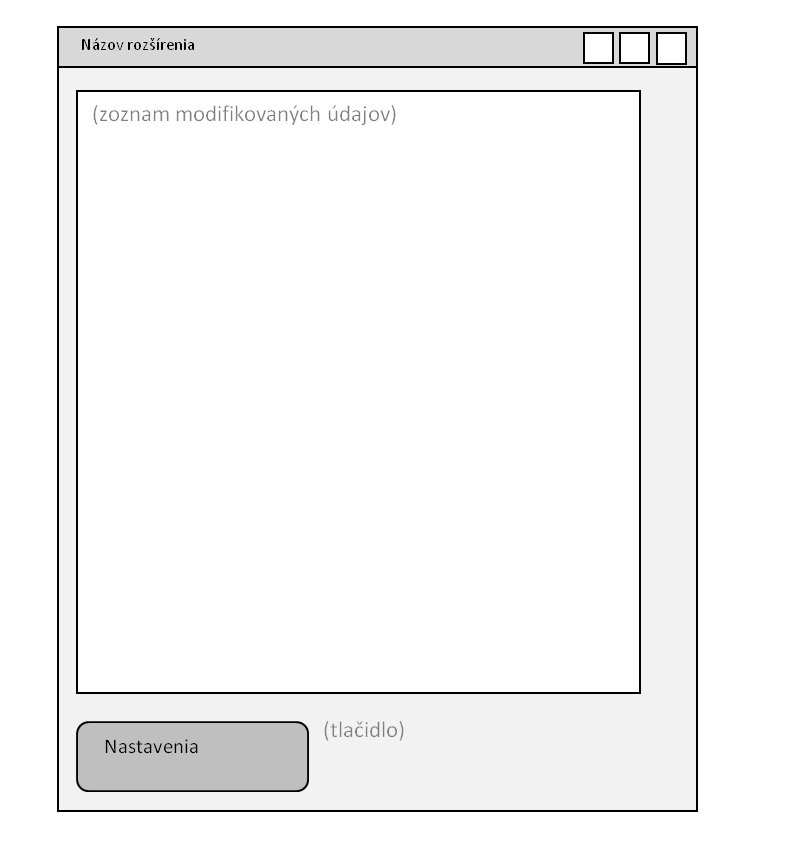
\includegraphics[width=8cm]{img/vzhlad.png}
%   \caption{Predpokladaný vzhľad rozšírenia.}
%   \label{vzhladobr}
% \end{figure}
% Dôležitou požiadavkou kladenou na rozšírenie bolo príjemné používateľské rozhranie~\cite{t00}. Z~tohto dôvodu malo rozšírenie obsahovať zoznam modifikovaných vlastností a~tlačidlo pre prístup k~nastaveniam rozšírenia v~jednoduchej a~praktickej forme. Predpokladaný vzhľad je zobrazený na obrázku č.~\ref{vzhladobr}.

% \begin{algorithm}
% \scriptsize
% \begin{algorithmic}
%  \STATE <text>
%  \IF{<condition>} \STATE {<text>} \ELSE \STATE{<text>} \ENDIF
%  \IF{<condition>} \STATE {<text>} \ELSIF{<condition>} \STATE{<text>} \ENDIF
%  \FOR{<condition>} \STATE {<text>} \ENDFOR
%  \FOR{<condition> \TO <condition> } \STATE {<text>} \ENDFOR
%  \FORALL{<condition>} \STATE{<text>} \ENDFOR
%  \WHILE{<condition>} \STATE{<text>} \ENDWHILE
%  \REPEAT \STATE{<text>} \UNTIL{<condition>}
%  \LOOP \STATE{<text>} \ENDLOOP
%  \REQUIRE <text>
%  \ENSURE <text>
%  \RETURN <text>
%  \PRINT <text>
%  \COMMENT{<text>}
%  \AND, \OR, \XOR, \NOT, \TO, \TRUE, \FALSE
% \end{algorithmic}
% \caption{Ukážka príkazov pre algorithmic}
% \label{alg:preview}
% \end{algorithm}

% \begin{lstlisting}[
%   caption={Ukážka výpisu programového kódu},
%   label={lst:main-c},
%   language=c,
%   style=code-listing
% ]
% /* Hello World program */

% #include<stdio.h>

% struct cpu_info {
%     long unsigned utime, ntime, stime, itime;
%     long unsigned iowtime, irqtime, sirqtime;
% };

% main()
% {
%     printf("Hello World");
% }
% \end{lstlisting}